\chapter{Methods}
In addition to the deployment of existing methods to achieve my research goals, this dissertation contains a number of innovations which are best described as methodological.  I include some of these innovations here, especially those of an extremely technical nature.  Some other methodological innovations, especially those of more interest to the computational neuroscience community, are reported later in the Results chapters.

\section{Approach to optimization using NeuronUnit}
Model optimization follows the following basic approach:
\begin{enumerate}
	\item Identify a model class whose parameters are to be optimized, e.g. the Izhikevich model.
	\item Identify a neuron whose experimental data will be used to guide optimization.
	\item Identify a suite of tests that can use that experimental data to guide the optimizer.
	\item Execute optimization of that model class against that suite of tests to return an optimized model.
\end{enumerate}
Within these steps are also a number of smaller decisions, including where the experimental data will be obtained and what kind of simulator will be used to run the model.
Using NeuronUnit, the steps above take the follow pseudo-code form:
\clearpage
\begin{lstlisting}[language=python]
# Import code from NeuronUnit
from sciunit import TestSuite
from neuronunit.models import MyModelClass
from neuronunit.tests import MyTestClass1, MyTestClass2, MyTestClass3
from neuronunit.data import get_data_from_database_x

# Get data about some neuron
neuron_type = "CA1 Pyramidal Cell"
neural_data = get_data_from_database_x(neuron_type)
test1 = MyTestClass1(neural_data[1])
test2 = MyTestClass2(neural_data[2])
test_suite = TestSuite([test1, test2])

# Optimize a model against this test suite
optimized_model = test_suite.optimize(MyModelClass)
\end{lstlisting}



\subsection{Novel Data Driven Optimization Constraints}

At the begging of my project the range of tests available for optimization in NeuronUnit was incomplete, initially tests in neurounuit were restricted to measurements of negative deflection in the membrane or the shapes of single action potentials. In order for model output to reflect the rich dynamics of experimental data, it was also necessary that the shapes and timing patterns of spike trains be assessed and tested. 

As noted in \ref{sec:data-sources} there where two experimental data types, each of which was used to constrain models differently: multiple spike shape features, and summarized electro-physiology reports. The distinction is important here because in the former case new feature extraction routines are needed, and in the second case it is not.

In order to obtain the first data type, I created an Allen cell-types API, the API allows one to create neuronunit tests from a data base of experimental cellular recording waveforms.

In order to create the new NeuronUnit tests, one must query the cell-types database, impose a new organization on the data, extract relevant features (EFEL), and convert model features to NeuronUnit tests. A similar API was created in order to render BlueBrain Project waveforms, eligible for NeuronUnit testing, such that the both the BlueBrain \cite{toledo} and Allen Cell-type data could then guide model fitting. %Tests obtained via the Allen API, were designed to execute inside a NeuronUnit and BluePyOpt frameworks.  

%experiment to NeuronUnit test
One can see the APIs being creating novel NeuronUnit tests here \url{https://github.com/fun-zoological-computing/BluePyOpt/blob/master/examples/bpo_nu_fusion/allen_efel_nu_deployed_tests_only-thesis.ipynb}
%Construction of tests from diverse experimental sources 
%My allen API is perhaps scattered. Allen API.
%Which is the best model.
In order to optimize reduced models, it was first necessary to develop optimizer-friendly implementations of these models. As described in methods, I developed three different optimizer friendly reduced models: Izhikevich model (spanning seven regimes), Adaptive Exponential Integrate and Fire model, and the GLIF model. Additionally I created one slower single compartment model and a I retrofitted a pre-existing multi-compartment conductance based models to make a broader array of comparisons across model types possible.

The range of tests available for optimization in NeuronUnit was also incomplete, especially as it focused on passive properties of the membrane or the shapes of single action potentials.  In order for model output to reflect experimental data, it was also necessary that the timing and patterns of action potentials be assessed and tested.  Therefore, I developed the ability for EFEL features to be calculated on NeuronUnit models. 


I developed the ability for EFEL features to be calculated on NeuronUnit models, as well as a new single test that measured and compared FISlope in Allen celltypes data. I organized these tests into new at threshold and above threshold Allen Data test sets. This required both the extraction of novel features and novel test types: (ISI, AHP-depth, adaption ratio etc.).   


Multi-core and or multi-threaded optimization requires that information about model properties be shareable across various processor threads. However, some common data types contain information that is not shareable between CPUs, and they must be translated into a globally sharable framework. I created a class Data Transport Container, that could contain be used to circulate only essential data, in a more shareable form. 

In order to both control optimization parameters and visualize optimization results, I also developed a web application, the application requires no programming skill to use, and it allows a user of the to select among multiple cell specific constraints, and multiple model types. %Once the user has specified enough parameters to define an optization job, the job can launch, and then return interactive results to the user when the optimization job is complete typically in minutes.


%\section{Approach to Optimization using NeuronUnit}
Model optimization follows the following basic approach:
\begin{enumerate}
	\item Identify a model class whose parameters are to be optimized, e.g. the Izhikevich model.
	\item Identify a neuron whose experimental data will be used to guide optimization.
	\item Identify a suite of tests that can use that experimental data to guide the optimizer.
	\item Execute optimization of that model class against that suite of tests to return an optimized model.
\end{enumerate}
Within these steps are also a number of smaller decisions, including where the experimental data will be obtained and what kind of simulator will be used to run the model.

Using NeuronUnit, the steps above take the follow pseudo-code form:

\begin{lstlisting}[language=python]
# Import code from NeuronUnit
from sciunit import TestSuite
from neuronunit.models import MyModelClass
from neuronunit.tests import MyTestClass1, MyTestClass2, MyTestClass3
from neuronunit.data import get_data_from_database_x

# Get data about my neuron
neuron_type = "Layer 5 pyramidal Neuron"
neural_data = get_data_from_database_x(neuron_type)
test1 = MyTestClass1(observation=neural_data)
test_suite = TestSuite([test1, test2, test3])
results = test_suite.optimize(model)
\end{lstlisting}

There are two different paradigms for evaluating models in NeuronUnit. Under the first paradigm the model is supported by NeuronUnit, and dynamic simulations of the model are present on the host computer and can be efficiently re-run.

Under the second paradigm the NeuronUnit version of the model only consists of model inputs and outputs that are streamed as needed from a different environment. This may be the case due to the complexity of the model, where re-implementing the model would not improve clarity. Or the full model may exist on a remote machine with outputs accessed via an API. 
%Another way of saying this is that if a "model" is simply a digitized set of waveforms, converting it to a model is as simple as labeling things such that NeuronUnit and the scientist are both consistent about what is a model and what isn't. 
The optimization procedures I describe in this work involve both paradigms, where optimizing within the second paradigm required dedicated code that is not supported within the previously described frameworks.

\section{Model Class Implementations}
Because optimization may involve an extremely large number of independent simulations of the same class of model, each varying only in model parameter values, it is critical that both the overhead for model instantiation and the duration of simulation be as low as possible. We built faster Python implementations of two neuronal models -- the Izhikevich model and the adaptive exponential integrate and fire model. My implementations of the Izhikevich model was based on an existing MATLAB forward Euler implementation, while my implementation of the adaptive exponential integrate and fire model came from vectorized Python code, which was relatively slow.

I was able to use a tool to make both of these models perform faster than the standard versions for the brian2 and NEURON simulators. This tool, \cite{numba}, enables Just In Time compilation (JIT).
 %Without over stating things, 
 When regarding this thesis effort and its contribution to knowledge, some of the value to the neuroscience modelling community comes from the implementation of these two fast Python neural model simulations. Because these simulations are written in Python, the code that implementations them is easy to understand share and execute, because the models are fast to dispatch they are useful in both network and optimization contexts where performance is critical. 
 
%A component of this work the Izhikevich model, I plan to push to the Open Source Brain %\href{https://github.com/russelljjarvis/IzhikevichModel.git}

\subsubsection{Why Existing Approaches Were Not workable}
In this research effort significant time was spent shoe-horning pre-existing tools into an optimization frame work, with limited success. These tools included:  PyNN, brain2, \emph{NEURON}, jNeuroML-2. However, several unexpected road blocks were encountered on the way.
 
When applying reduced models to optimization, there was a cluster of known errors and limitations in pre-existing community standard reduced model simulators. 

To make optimization of models tractable it was important to do ongoing feasibility testing. For example its important to evaluate the the utility of established model implementations, as using these models to optimize may not in fact be feasible.\\ 
Despite an a large number of choices of FOSS reduced model implementations, many off the shelf implementations were not useful, or significant intervention was required to make some established implementations workable inside an optimization framework. \\
 
Some revisions to the Izhikevich model include equation tweaks, in order to let cells better reproduce in-vivo firing dynamics, such as bursting, and re-bound spiking \url{https://github.com/OpenSourceBrain/IzhikevichModel/blob/master/MATLAB/izhi2007.m}. However, when multiple equations, however closely related, are incorporated under the same umbrella, this fractures the implementation of the model into sub-models. The \emph{NEURON} implementation of the Izhikevich model is fractured. There are different implementations for different regimes. This meant that switching between model regimes during optimization would be a non-trivial exercise because the is already splintered between two languages (NEURON, NMODL, python), the source code would be highly complicated such that it would not be readable, and it would loose generality, overly customized towards one target model. The NEURON code, needed NMODL files to be compiled for each different regime, and promised performance of the C based NEURON library was not actualized. The only benefit to using this model, was that its parameter ranges are well tested and understood within OSB and NeuroML-2 community.

Because the PyNN implementations of the Izhikevich models are "wrapped" versions of essentially NEURON models, PyNN models still retained the disadvantages of the NEURON models (surprisingly poor speed on the Izhikevich model) while introducing other problems. PyNN is designed to preference the description and implementation network simulations. A data-type called a "lazy-array" is the smallest elemental container for neuron models in PyNN, but it is meant to store populations of neurons as opposed to single neurons, as such the lazy-array often slows down and gets in the way of the single neuron simulations, which model fitting depends on.
%(lazy array evaluation). 

 Sub models $[1-3]$ are really different parameterizations of the same equation, sub-models $[4-7]$ are actually different equations, meaning that there is a total of $4$ Izhikevich sub-models. To permit optimizer access to the broadest range of Izhikevich dynamics, a new meta-parameter $cell_type$, was created. This number ranging $[3-7]$ (unique model equations included only), allows the optimizer to change which Izhikevich sub-model it samples from. Later in on in results, we see that in fact even when fitting to static electrical properties, optimizer access to the broader set of firing regimes improved the quality of fits.


%The described limitations of the 
%https://github.com/NeuralEnsemble/PyNN/issues/370$%}, journal={GitHub}, author={Davison A}
%}


%@misc{neuralensembleadexp, title={pyNN.neuron %implementation of AdExp is unstable, gives poor results  Issue $#266 · NeuralEnsemble/PyNN$}, url={$https://github.com/NeuralEnsemble/PyNN/issues/266$}, journal={GitHub}, author={Davison A.}
%}
\url{https://github.com/NeuralEnsemble/PyNN/issues/370} 
%\cite{neuralensemble_adexp}
\url{https://github.com/NeuralEnsemble/PyNN/issues/266} 
%\cite{neuralensemble_adexp2}
 
A constant error warning plagued brian2 investmentallations was.
\begin{verbatim}
Brian2 causes error:
 ERROR      Brian 2 encountered an unexpected error. If you think this is bug in Brian 2, please report this issue either to the mailing list at <http://groups.google.com/group/brian-development/>, or to the issue tracker at <https://github.com/brian-team/brian2/issues>. Please include this file with debug information in your report: /tmp/brian_debug_t0acbm4l.log  Additionally, you can also include a copy of the script that was run, available at: /tmp/brian_script_juzhsbph.py Thanks! [brian2]
Traceback (most recent call last):
\end{verbatim}
In two classes of model a feasible choice of implementation did not exist and it was easier to re-implement those models. The two models I re-implemented were
the Adaptive Exponential Integrate and fire Model, and also the IZHI
model.  In the work below, I profile existing model implementations, and
justify the reasons for re-implementing.\\
\\
This is in contrast to the brian2/neuraldynamics AdExp model, which took
between 2 or 3 times longer to find a rheobase current injection value. However the slowness is not caused by the simulation backend (brian2 which is relatively fast and efficient). The slow down is caused by the way the model is defined. Specifically the
model is defined in a middle code layer neurodynamics \cite{gerstner2014neuronal}.\\
\\
It is very likely, that the model implementation is correct, since Gerstner is an author of one of the original adaptive exponential publications, and the neural dynamics book that the brian2 code is strongly affiliated with. Since Integrate and Fire models don't formally include spikes when an implementation does include spikes, it is an optional add on.\\
\\
The AdExp neurodynamics models default implementation causes spikes with peaks below $0mV$, since the IZHI model like all integrate and fire models do not explicitly include spikes\\
\\
This is not technically wrong, but it violates
assumptions in the \emph{NeuronUnit} feature extraction protocol. The default spiking behavior, looks odd, and it is simply this poor model definition that is causing a slower optimizer performance. The optimizer takes an unusual waveform shape, and searches for longer in distant
parameter regions to find a good fit.\\
\\
Over the course of evaluating the brian neural dynamics model \cite{gerstner2014neuronal}. I experienced some phenomena that only occurred in the context of genetic algorithm optimization. The reason why optimization provides a different evaluation context is because, in optimization simulation objects are required to be created and destroyed rapidly and on mass. Brian2 is designed to be an efficient network simulator, the case of being designed for network simulation, may assume you will want to create a lot of neural models that persist efficiently together in memory (this was also a problem with PyNN models). Therefore you might see below, that while only one brian model exists in memory, performance is okay, but when creating and destroying models rapidly and on mass a slow down occurs.\\
\\
Below I have implemented a Python integrator for the adaptive exponential integrate and fire model. This solver led to faster evaluations of current injection experiments. The integrator I developed has a $0mV$ spike when evaluated at default parameter values.\\

Brian2 and SciUnit sometimes collided in name space and logging.
%\href{https://github.com/scidash/sciunit/pull/124/files/83907ba68740642178ebb91084f6e382e06a43c4#diff-d68791d2ed5dfaa96a900be6180bd950}

\section{Profiling the JIT Enabled AdExp Model}
Mean time taken on single model evaluation:$ 0.0012554397583007812s $
Mean time taken to compute Rheobase:
$0.183s $
This was slightly faster than Izhikevich implementation which was for total rheobase solution $ 0.462s $ and $  0.002 s$ per run. Solving for Rheobase takes a average of 15 model evaluations.
%\begin{figure}    
%\begin{center}
%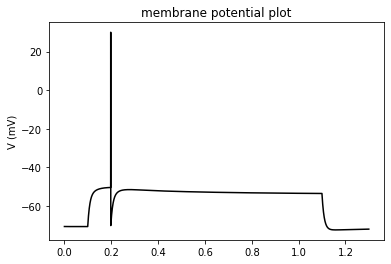
\includegraphics[width=0.25\linewidth]{figures/backend_check_files/backend_check_6_2.png}
%\caption{}

%\end{center}
%\end{figure}

%\begin{verbatim}
%    251 ms +- 5.02 ms per loop (mean +- std. dev. of 2 runs, 1 loop each)
%    240 ms +- 11.1 ms per loop (mean +- std. dev. of 2 runs, 1 loop each)
%    223 ms +- 12.5 ms per loop (mean +- std. dev. of 2 runs, 1 loop each)
%\end{verbatim}

\begin{verbatim}
    922 ms +- 12.7 ms per loop (mean +- std. dev. of 7 runs, 1 loop each)
\end{verbatim}

\subsection{Comparison of Parallel and Serial Speeds and Accuracy}

Below is the Brian2/NeuralDynamics AdExp model. In-order to make the spike height greater than $0mV$ it was easier to use computer code to schedule waveform modifications that occur straight after the the brian2 simulation, these scheduled waveform modifications can be considered part of a peripheral shell of simulation code. In postprocessing
the waveform data type is a Neo Wave form object that is artificially the algorithm of determining rheobase and displaying results. The time of this model is determined on multiple factors, as discussed elsewhere, execution time is not uniform across model parameterizations. Models with multispiking behavior will take longer to solve.

Simulation times for this model vary, dramatically possibly because of
lazy evaluation, the simulation times may vary according to what else
you are running on your computer. Not all models experience a speed up when executed in parallel, however
this model was faster in the parallel Rheobase determination algorithm. Some common times are: $3.92,6.75,4.48,5.17$. Mean time was:

\subsection{Comparison of Time to Find Rheobase}

Custom implementation JIT enabled implementation: $4.0s$. 
Brian2 taken to find Rheobase: $4.40s$ (serial), $3.976s$ (parallel).

The evaluation times between Brian2 and the custom written
integrator are similar. Both have average rheobase solution times of approximately 4 seconds, however the spike shape derived from the custom written integrator look more realistic under default paramaterizations. The biological plausibility of default model paramaterization has consequences for model optimization speed, because when  models undergo mutation and cross-over the mean of random models regressors towards the default model initialization, and if the default model is a bad fit to data, the average model sampled by the genetic algorithm will also be bad to data.\\

\begin{figure}
\centering
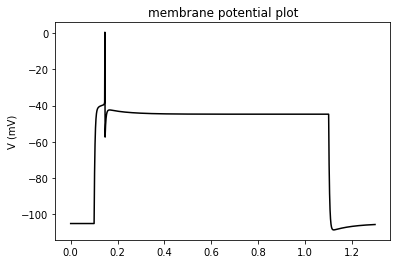
\includegraphics[scale=0.45]{figures/backend_check_files/backend_check_12_10}
\caption{Model Parameterization of the brian2 Simulator with the customization: interpolated spike height, forced to be above $0mV$}
\label{fig:sub1}
\end{figure}

\begin{figure}
\centering
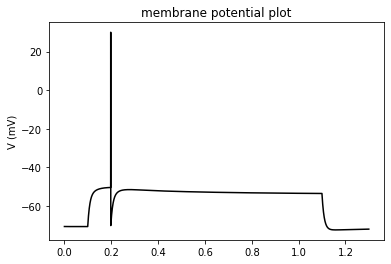
\includegraphics[scale=0.45]{figures/backend_check_files/backend_check_4_2}
\caption{Default model parameterization of the custom written integrator}
\label{fig:sub2}
\caption{Comparison between two Adxaptive Exponential Implementations}
\label{fig:test}
\end{figure}




    
$272 ms +- 66.5 $/mu$s per loop (mean +- std. dev. of 2 runs, 1$ loop each)

The next model to be evaluated is the NEURON Izhikevich model. The NEURON Izhikevich model has various draw backs. 1. It depends on an external file which must be recompiled each time this project is recreated. 2. The build environment of NEURON is non-trivial, and only a super dedicated NEURON modeller would install it on their system. Any performance advantage of using NEURON investment does not exceed the installation cost of installing the program. 3. The model implementation code is less generalizable than than the published Izhikevich model itself. Where the standard NEURON-NeuroML code only covers the Regular-Spiking model * This is likely due to a name space conflict between Capacitance. Neuron has a `capacitive' mechanism inside modelled Neurons, this particular model has section capacitance as well as an introduced capacitive term inside a C-compiled mechanism. Both contribute to a the membrane
potential calculation. * The NEURON Izhi model took $78$ seconds to find the rheobase current injection value $ 51.79367065 * pA $.

    
%\begin{center}
 %   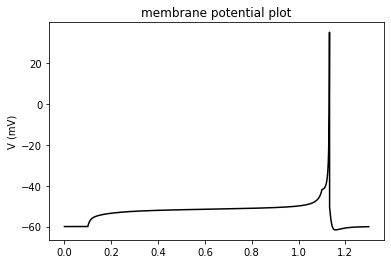
\includegraphics[width=0.7\textwidth,]{chapters/figures/backend_check_files/backend_check_14_2.png}
%    \caption{where is picture}
%\end{center}


%\begin{figure}
%    \centering
%    \includegraphics{chapters/normal_distribution}
%    \caption{This is your image%}
%    \label{fig:my_label}
%\end{figure}
%A tool numba JIT

% https://www.overleaf.com/learn/how-to/Images_not_showing_up 

        
The enabled forward Euler python Izhikevich model was very fast. The forward euler
implementation utilized Numba JIT \cite{lam2015numba}. Rheobase is found in under a second,
and in many cases close 0.5 seconds. This represents a very dramatic
speed up. Unlike the NEURON NeuroML implementation of the izhikitich equation,
this implementation is just as generalizable as the original MATLAB
implementation of the Izhikevich model, because it was possible to unify the fractured implementations in the one python simulator backend.

\subsection{NEURON+Python single compartment Conductance Model.}

Conductance based models took approximately the same amount of time to evaluate the Rheobase search algorithm as the python implementation.

The author also engineered GLIF model support for $NeuronUnit$ tests. In practice these models where hard to configure without expert knowledge, GLIF models contain the most parameters of all models, and many of these parameters are multi dimensional. GLIF models do not by necessity spike, interpolated spike times, are added in however, it does not make sense to evaluate GLIF models on spike shape features.

It is worth noting that the layer 5 neocortical pyramidal neuron was very slow to dispatch relative to the reduced models developed in this thesis work. Where as a typical reduced model described here evaluated in the order of $2.5 ms$, this model on average took $5.74$s, for a single run and $34.8$s to solve for the models Rheobase, current. To be fair, the model was run without activating NEURONs variable time step cvode. However, even with variable time step applied to the differential equation solver the magnitude of the disparity is still still several $seconds:$ several $ ms$. 

% time taken to compute rheobase $ 12.6s $


%\begin{verbatim}
%  time taken on
%  block 0.6859951019287109 \textbackslash{}n3.3 ms +- 9.79 %$\mu$s per loop (mean +- std. dev. of 2
%  runs, 100 loops each)\textbackslash{}n3.32 ms +- 30.9 us per loop (mean +- std. dev. of 2 runs,
%  100 loops each)\textbackslash{}n3.19 ms +- 10.9 us per loop (mean +- std. dev. of 2 runs, 100
%\end{verbatim}
        


%This problem in the default parameterization of the python model was later located in the scale or units of capacitance, if default capacitance parameterization is multiplied by 100.0 the problem goes away.


%\begin{center}
%\includegraphics{figures/backend_check_files/backen%d_check_22_2}
%\end{center}

%$ 1.40762329 * pA $


% \subsection{NEURON versions of single compartment Conducance
% model.}

% Took $8.57$ seconds to find Rheobase.

%Hodgkin Huxley Conductance based channels models took approximately the same amount of time to evaluate the Rheobase search algorithm as the python implementation.

%The NEURON implementation was slightly faster, and the default parameterization of the model lacked `ringing'', or below threshold oscillations that the Python ODE version had under default conditions.

%This problem in the default parameterization of the python model was later located in the scale or units of capacitance, if default capacitance parameterization is multiplied by 100.0 the problem goes away.


%which makes debugging their behavior very difficult. %None the less GLIF models where among the fastest to evaluate, and the author had success in making fitting these models to Allen Rheobase data.

    %\graphicspath{ {../figures/} }
%    \begin{center}
%    \begin{figure}
%    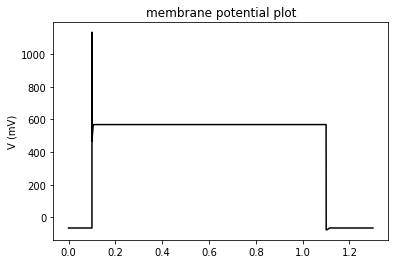
\includegraphics{figures/backend_check_files/backend_check_26_2}
    %kend_check_files/backend_check_26_2.png}
%    \end{figure}
    
%    \end{center}
%\begin{verbatim}
% 112.5 pA
%'value': array(1.40645904) * pA
%\end{verbatim}

% parameters of an adaptive exponential model
%\begin{verbatim}
%\{'El\_reference': -0.07016548013687134, %'C': 3.990452661875942e-10%,
%'init\_threshold': 0.02964956889477108, %'th\_inf': 0.02964956889477108,
%'spike\_cut\_length': 109.5, %'init\_voltage': -35.0, 'R\_input': %910258965.9792937\}
%\end{verbatim}
%$ Rheobase = 112.5pA $
%time taken to execute GLIF model when deliberately undersampling to save time.
%$ 0.23476457595825195 $

    


%$ 112.5 pA $
%$0.0 mV$ $-0.065 mV$

%    \begin{verbatim}
%    \{'value': array(183.33333333) * pA\}
%    \end{verbatim}

%\begin{verbatim}
%array(112.5) * pA
%\end{verbatim}


%\begin{verbatim}
%    0.017240506310425608 mV -0.08583939747094235 mV
%    0.017240506310425608 mV% -0.08583939747094235 mV
%\end{verbatim}

    %\begin{center}
    %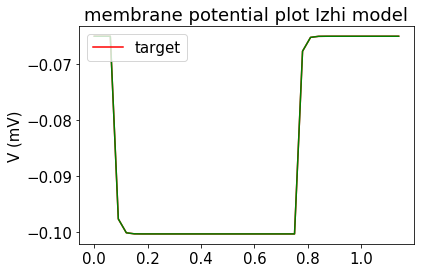
\includegraphics{figures/backend_check%_files/backend_check_32_2.png}
    %\end{center}

%\input{chapters/methods/rheobase}

\section{Pre-Existing Model Class Implementations}
First I accessed an implementation of the Izhikevich model that was translated from jNEUROML into a NEURON simulator implementation.
However, this implementation fragmented the family of Izhikevich models into chattering and non-chattering subtypes.
The model implementation also seemed to have an internal conflict between two capacitive terms and could not reproduce all of the original publication figures.
Although the NEURON simulator is designed to be fast, there is a cost associated with reloading the NEURON environment many times in fast succession, and implementation odel execution times were not brief enough to be useful for optimization.

\section{Other Model Class Implementations}
For various reasons described in detail below, existing implementations of some models were not adequate for this research.
These reasons included speed, generality, and consistency.

\subsection{Model Execution: The Need for Speed}
Because optimization may involve an extremely large number of independent simulations of the same class of model, each varying only in model parameter values, it is critical that both time costs--both the overhead for model instantiation and the duration of simulation itself--be as low as possible.
Existing modeling tools contain overhead associated with model initialization and shuttling results in memory.
These costs are trivial for single simulations, but begin to add up in optimization runs of thousands or even millions of simulations.  
Even the marginal cost of simulation--expressed as seconds on a wall clock per seconds of model output simulated--is often slower than expected using existing tools, due to some of these tools being written to accommodate more complex, biophysical models, rather than engineered for raw speed.
During optimization, many parameter sets are explored, and the speed of  simulation can be determined by the parameter values.
For example, those parameter sets which produce many spikes in a given simulation run more slowly, because $\frac{dV_{M}}{dt}$ changes rapidly throughout the simulation, necessitating reductions in simulation step size to avoid numerical instability.

\subsection{Model Design: Lack of Generality}
Significant time was spent in the early years of this project shoe-horning pre-existing tools into the desired optimization framework, with limited success.
These tools included, among others, model designers and neural simulators such as PyNN, Brian2, NEURON, and jNeuroML.
However, several unexpected road blocks were encountered on the way.

\subsubsection{NEURON}
The NEURON simulator is a very mature and respected neuron and neural network modelling framework \citep{carnevale2006neuron}. This simulator specializes in multi-compartment conductance based models of neurons and neuronal networks, but the simulator has also been made to accommodate many reduced model implementations. The NEURON implementation of the Izhikevich model is fractured in that there are different NEURON NMODL implementations of the equations for different parameter regimes.

When running only a single model simulation this is not much of a problem. However, switching between Izhikevich model regimes during optimization (as would occur when a parameter value crossed a regime boundary) is a non-trivial exercise.
Even if successful, any multi-language source code successfully implementing this would be complicated, unreadable, and lack generality.
Specifically, NEURON requires NMODL files to be compiled for each different regime, and it may be difficult to know in advance which regimes the optimizer is likely to sample from.
Additionally, the promise of fast performance due to the C-based NEURON library is not actualized with this model.
Because NEURON is well-understood within the OSB and NeuroML community, I used it only to produce reference simulations to verify that the output of my model implementations were in fact accurate according to community standards.

\subsubsection{PyNN}
PyNN provides the convenience of working in Python, and with a convenient procedural interface for model design and execution \citep{davison2009pynn}.
However, its implementations of most reduced models (e.g. Izhikevich) are simply ``wrapped" versions of NEURON models; consequently PyNN has the same disadvantages as NEURON.
PyNN is also designed with network simulations in mind, which means its designers have chosen performance trade-offs that favor network simulations over single neuron simulations.
For example, a data-type called the ``lazy-array" is the most elemental container for neuron models in PyNN, but it is meant to store populations of neurons as opposed to single neurons;
as such the lazy-array adds overhead to accessing single model results.

% in slow single neuron simulations.

Additionally, the NEURON implementations that underlie the PyNN-provided AdEx and Izhikevich model classes suffer from some fidelity issues under certain regimes and parameter sets, compromising optimization quality (see \cite{neuralensembleadexp2, neuralensembleadexp} for details).

\subsubsection{Brian2}
Brian2 \citep{stimberg2019brian} is, in principle, an excellent simulator for working with reduced neuron models, as it allows for differential equations to be expressed in an intuitive form, while also keeping track of dimensions and units.
However, it may not be mature enough for complex applications, as it produced errors in optimization contexts that did not occur during routine simulation of single-parameter sets.

Even when these errors did not occur, (e.g. using the Brian2 AdExp model), certain optimization steps (such as identifying the rheobase current for a given set of model parameters) took 2-3 times more simulation time then a reference approach (described in the next section).
This slowness was not caused by the simulation mechanics themselves (Brian2 is relatively fast and efficient, as described in \cite{stimberg2019brian}.)
Instead, these delays are caused by the way the model is internally defined, specifically using a
so-called ``neurodynamics" layer \citep{gerstner2014neuronal}.

While it is very likely that this implementation is useful and correct in many contexts (Gerstner is an author of one of the original AdEx model publications \citep{brette2005adaptive}, and the Brian2 implementation is derived directly from his work), it is problematic for the feature extraction step required in optimization.
Specifically, these implementations do not formally contain any notion of ``overshooting" spikes, since when the spike threshold is reached, the membrane potential is simply set to some reset value; the presence and timing of a spike is recorded only when a separate process is explicitly set to watch for such an event.
This is not technically wrong, but it violates a key assumption in the \emph{NeuronUnit} feature extraction protocol (the existence of an action potential waveform to extract), and the extra layer for detection of spiking adds computational overhead.
Imputing a spike-like waveform near threshold can help solve the problem, but then optimization results and performance becomes contingent on the design of this waveform imputation, and not on the model itself.

Lastly, over the course of evaluating the Brian neural dynamics model \citep{gerstner2014neuronal}, I encountered some problems specific to genetic algorithm optimization.
This context is not identical to simply running a series of simulations in series, because optimization operates in parallel, must fit into computer memory, and thus requires that simulation objects be created, simulated, and then destroyed rapidly and en masse.
Since Brian2 was designed for stability, is was not designed to make model disposal computationally efficient (the problem of clearing objects from memory efficiently is, from a computer science perspective, trickier than it might initially sound).
Therefore, performance of Brian2 suffered when I re-purposed its code to work in an optimization context.
Brian2 does support its own internal scheme for model fitting \citep{brian2modelfitting}, however this scheme was only published late in this thesis work, and it is unknown what technical tricks they employed to enforce model garbage collection. 
Additionally this scheme is highly divergent from the multi-objective DEAP framework described in Section \ref{sec:tech-details}, so it is not readily interoperable with the model fitting workflow described here.

\subsubsection{My Approach}
\label{sec:new-models}
In summary, despite several choices for existing, free, open-source software (FOSS) reduced model
implementations, these implementations were not useful, or significant intervention would have been required to apply them within an optimization framework.
To overcome this and accelerate optimization, I built faster ``direct" implementations of two neuronal models (the Izhikevich model and the AdEx model).
One of the these was inspired from the existing MATLAB forward Euler implementation of the Izhikevich model, while the other was adapted from an existing Python implementation of the AdEx model using vectorized code.
While neither of these was especially fast, they provided the basic recipe upon which a faster Python implementation could be built.
Do note that the purpose of these new implementations was not model exploration, analysis, or sharing; existing tools are adequate for these purposes.
The purpose of the new implementations was simply to make large optimization runs computationally tractable.

Although typically much faster than R, Python does not have a reputation for speed; implementation details have a large impact on performance.
Therefore, I used a tool called Numba \citep{lam2015numba} that enables Just-In-Time compilation (JIT) of Python code, making it comparable in speed to compiled C code.
This tool cannot be applied to any arbitrary Python code, so functions to which it is applied must be designed with only a fairly plain subset of the usual syntax and library of Python.
In other words, it cannot be used to simply speed up any pre-existing Python code.
%all code is hand-coded, even cutting and pasting is done by hand suggested synonym crafted.
I crafted the two model types above to be JIT-compliant, with the result that both became significantly faster than analogous models using NEURON or Brian2 simulators.
Importantly, simulation outputs retained a binary near-match in all cases, confirming that nothing was lost in the course of gaining this performance improvement.
I used these new implementations extensively throughout the project, and they are available to others at \cite{jithub}. 
The code that implements them is fairly easy to understand, share, and execute, and I hope they may be useful to others who have similar performance needs, either for optimization contexts or in large network models on generic commodity computer hardware where small performance gains are worth chasing. 

Some models were executed in their native implementations using the NEURON simulator with an adaptive time step.
After each model run, the variable time step vectors were resampled into fixed time step vectors using interpolation.
I accelerated this inherently slow process by applying the JIT framework to prior code contributed by a colleague \citep{birgiolas2019towards}.

Below, I profile my implementations and compare them to the existing FOSS implementations.
My implementations led to faster per-simulation evaluations of simulations involving somatic current injection. 
Furthermore, my implementation exhibited over-shooting spikes (spikes crossing 0 mV, as occurs in real neurons), making them more compatible with NeuronUnit feature extraction.

\subsection{Profiling the Models}
Obtaining the rheobase of a model for a single parameter set requires simulating it many times at different values of somatic current injection until the minimum action-potential inducing current is obtained (to within some tolerance; here I used 0.1 pA, near the standard deviation of thermal noise).
This takes 10-15 simulations, on average.
\begin{verbatim}
My AdExp implementation:
Single model simulation: 0.00126 s
Rheobase computation: 0.183 s

My Izhikevich implementation:
Single model simulation: 0.002 s
Rheobase computation: 0.462 s
\end{verbatim}

\subsubsection{Comparison of Speed and Accuracy Versus Brian2}
In-order to implement NeuronUnit-compatible Brian2 AdEx model simulations, I imputed spike waveforms (at recorded spike locations) immediately following each simulation.
The simulation time of this model is determined by multiple factors, as discussed elsewhere. Execution time is also not uniform across model parameterizations; in particular, parameter sets exhibiting more spikes take longer to solve numerically.
I compared this with the same parameter sets in my implementation, with the results shown below:

A large fraction of the time spent simulating models under a single set of parameters is spent obtaining the rheobase current, upon which several subsequent tests and extracted features depend.

The JIT implementation of the AdExp model was approximately 1000$\times$ faster than the Brian2 model.
Another benefit of the JIT implementation was that it did not require imputation of action potential waveforms (as was required for the Brian2 implementation); without additional work, the JIT implementation produced much more realistic-looking action potential waveforms under most model parameterizations.
To the extent that action potential shape is an optimization target, this is a decisive advantage for the JIT implementation.

\begin{figure}[!htb]
\begin{center}
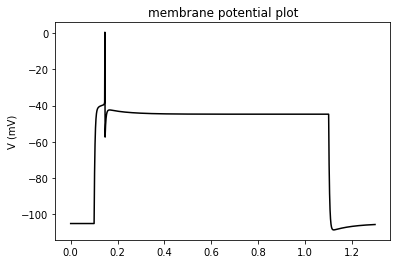
\includegraphics[scale=0.7]{figures/backend_check_files/backend_check_12_10.png}
\caption[Brian2 simulation of the AdEx Model]{\textbf{Brian2 Simulation of the AdEx Model.} Simulated membrane potential trace from the AdEx model at rheobase using the Brian2 simulator. The action potential waveform has been interpolated at the time when the simulator reported a spike.
The horizontal axis shows time in seconds.}
\label{fig:AdEx-Brian2-sim}
\end{center}
\end{figure}

\begin{figure}[!htb]
\begin{center}
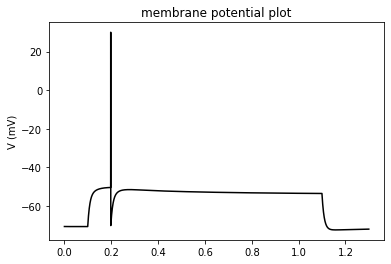
\includegraphics[scale=0.7]{figures/backend_check_files/backend_check_4_2.png}
\caption[JIT Simulation of the AdEx Model]{\textbf{JIT Simulation of the AdEx Model.} Simulated membrane potential trace from the AdEx model at rheobase using my JIT implementation. In contrast to Fig. \ref{fig:AdEx-Brian2-sim}, the dynamics of the action potential arise naturally from the integrated equations and do not require interpolation.}
\label{fig:AdEx-JIT-sim}
\end{center}
\end{figure}

\subsubsection{Comparison of Speed and Accuracy vs NEURON}
I also compared the performance of my implementation of the Izhikevich model to the one generated by NEURON from the OpenSourceBrain Izhikevich model NeuroML2 files.
This NEURON implementation has several drawbacks, including: 1) It depends on an external file which must be recompiled each time this project is recreated; 2) The build environment of NEURON is non-trivial; 3) The model implementation code is less generalizable than than the published Izhikevich model itself.
For example, the standard NEURON-NeuroML2 code only covers the Regular-Spiking flavors of this model, and does not support the full range of model parameterizations; 4) Name space conflicts between built-in NEURON parameters and Izhikevich model parameters.  

%\begin{center}
 %   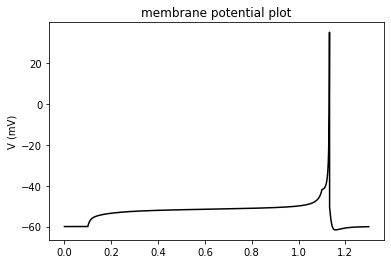
\includegraphics[width=0.7\textwidth,]{chapters/figures/backend_check_files/backend_check_14_2.png}
%    \caption{where is picture}
%\end{center}


%\begin{figure}
%    \centering
%    \includegraphics{chapters/normal_distribution}
%    \caption{This is your image%}
%    \label{fig:my_label}
%\end{figure}
%A tool numba JIT

% https://www.overleaf.com/learn/how-to/Images_not_showing_up 
        
The NEURON implementation of the Izhikevich model took $78$ seconds to identify the rheobase current.
In contrast, my implementation identified the rheobase in only $\tilde 0.5 s$.
This represents a very dramatic speed up, which can largely be attributed to overhead associated with initializing successive simulations.
Furthermore, my implementation generalizes to all possible parameter values for the Izhikevich model parameters, thus allowing for all of the many diverse spiking behaviors exhibited in the original publication by \cite{izhikevich2003simple}.

%\begin{verbatim}
%  time taken on
%  block 0.6859951019287109 \textbackslash{}n3.3 ms +- 9.79 %$\mu$s per loop (mean +- std. dev. of 2
%  runs, 100 loops each)\textbackslash{}n3.32 ms +- 30.9 us per loop (mean +- std. dev. of 2 runs,
%  100 loops each)\textbackslash{}n3.19 ms +- 10.9 us per loop (mean +- std. dev. of 2 runs, 100
%\end{verbatim}
        
%\subsubsection{Comparison of speed and accuracy vs NEURON for %conductance-based models}
%Could the relatively poor performance of existing implementations 5above be due the use of reduced models?
%I ran similar profiling exercises for a single-compartment %conductance-based model (implementing the Hodgkin-Huxley equations %\cite{rall1962electrophysiology}) to see whether the disparities %above persisted.
%I compared an existing Python implementation for simulation of %this model against the NEURON implementation.
%Conductance-based models took approximately the same amount of
%time ($12.6 s$ XXXX put in exact numbers) to determine the %rheobase as the existing Python
%implementation, suggesting that . XXXX What is this comparison?  %Conductance-based vs Python?

%\begin{center}
%\includegraphics{figures/backend_check_files/backen%d_check_22_2}
%\end{center}

%$ 1.40762329 * pA $
%XXXX Redundant? Hodgkin Huxley Conductance based channels models %took approximately the same amount of time to evaluate the %Rheobase search algorithm as the python implementation.

%The NEURON implementation was slightly faster, and the default parameterization of the model lacked `ringing'', or below threshold oscillations that the Python ODE version had under default conditions.

%This problem in the default parameterization of the python model was later located in the scale or units of capacitance, if default capacitance parameterization is multiplied by 100.0 the problem goes away.

%    \begin{verbatim}
%time taken on block 8.573923826217651
%    \end{verbatim}

\subsubsection{The GLIF Model: a Limited Model}
Although GLIF models are intentionally limited in behavior to below threshold firing dynamics, these models are still relevant to the neuronal modelling community.
I developed a Generalized Leaky Integrate-and-Fire (GLIF) model by manipulating some pre-existing code until it was interoperable with the NeuronUnit framework.
Because GLIF models do not include spike waveforms (like the AdEx implementations discussed above), imputation of these waveforms is required for broad spike shape optimization.
GLIF models are not particularly fast, nor have they historically been good at predicting  spike timing in neurons \cite{teeter2018generalized}.
However, GLIF models are widely-used within the Allen Institute, with that organization providing cell-specific GLIF models for each neuron that they record.
So I included them here for completeness and for comparison to previous work.

%. In practice this class of reduced models is difficult configure without expert knowledge, since it contain more parameters than its competitors, and many of these parameters are vector- rather than scalar-valued.
%Nonetheless, GLIF models were problematic moderately fast with $dt$ set to $5e-3 seconds $ which is 1000 times the recommended 5e-6 seconds, which is offensively slow, and I used these successfully to optimize models against data provided by the Allen Institute (see XXXX section in Results).
%$ Rheobase = 112.5pA $

\section{Parallel Rheobase Determination}\label{sec:parallel-rheobase}
In the preceding section, I discussed determination of the rheobase of a model as one of most computationally expensive steps in evaluating a given set of model parameters. 

\subsection{Why is the Rheobase Important?}
The rheobase is defined as the minimum current required to elicit at least one action potential.
In slice physiology experiments, this usually means a square pulse of somatically-injected current lasting for a fixed amount of time, for example $500 ms$.
The rheobase not only characterizes the excitability of a cell, but it also serves as a landmark or anchor for computing many other features of a cell's suprathreshold behavior.
For example, once the rheobase is known, one can compute a so-called "FI curve" -- the number or frequency of action potentials in response to a given amount of injected current -- at fixed multiples of the rheobase, providing a compact summary of excitability.
Both the Allen Institute and the Blue Brain Project use such rheobase-linked excitability measures.
The rheobase current can also be used to compute features of spike waveforms.
These features may vary with the amount of injected current, because the rising phase of an action potential may include both sodium current and pipette currents.
By using the rheobase current, this latter confound is minimized because the patch pipette current is roughly offset by outward currents (were the pipette current any less, the outward currents would have prevented a spike, by the definition of rheobase).
Consequently, action potential waveform features like threshold, width, and height are often performed at the rheobase current.

\subsection{How is the Rheobase Determined?}
Determining the rheobase involves repeated application of a more general algorithm that runs one simulation to determining the number of action potentials evoked by a particular magnitude and duration of somatic current injection.
Because the rheobase value partitions suprathreshold stimulus amplitudes from subthreshold ones, its determination can be accelerated by treating as a search tree problem.
In a search tree, the search space is adaptively narrowed between two endpoints until a target is identified.
For the rheobase, this means asking (1) "What is maximum current injected so far that resulted in zero spikes?" and (2) "What is the minimum current so far that resulted in one or more spikes?" and then running a simulation at some current amplitude in between those two values (e.g. halfway between in the case of a binary search tree).

\subsubsection{Serial rheobase determination}
The procedure above can be run in serial (i.e one simulation after another) until the rheobase is narrowed down to an acceptably narrow range, e.g. +/- 1 pA.
The initial search begins with no knowledge of any minimum suprathreshold or maximum subthreshold current amplitudes, so I use the starting range 300 pA to -100 pA, respectively.
A binary search is applied within this space, with additional code to handle edge cases outside this range.
Ignoring those edge cases, such a binary search requires $log_2(I/i)$ simulations, where $I$ is the range being searched (here, 400 pA) and $i$ is the resolution of the solution (here, 1 pA).
Thus, ~9 simulations are required to obtain the rheobase using this binary search strategy.

\subsubsection{Parallel rheobase determination}
This process can be accelerated by running simulations in parallel.
While each step of the search requires knowledge of the outcomes of the previous simulations (and so there can be no parallelism across steps, other than brute force parallel search of the entire range of currents, which is extremely inefficient), it is possible to parallelize within each step.
A binary search partitions the search space in two by simulating a current injection at $(sub+super)/2$ pA, where $sub$ is the previous maximum subthreshold current, and $super$ is the previous minimum suprathreshold current.
The value $(sub+super)/2$ pA either does or does not produce a spike, leading to its value being used to update either $super$ or $sub$, respectively.
The search space is cut in half, so this simulation effectively generates one additional bit of information about the amplitude of the rheobase.
This repeats ~9 times until all 9 bits of uncertainty (from the initial 400 pA) range have been eliminated.
Parallelism accelerate this by applying an N-ary search (rather than a binary search), where N is the number of parallel processes, and N+1 the number of regions of current amplitude to search.
This is described in Figure \ref{fig:rheobase}.
Consider the initial 400 pA range.
With only one thread, this range is bisected and a simulation run at it midpoint $(-100 pA + 300 pA)/2 = 100 pA$.
With seven threads, this range can be octo-sected, with concurrent simulations run at each of seven values, i.e. ${-50, 0, 50, ..., 300, 350}$ pA.
The highest of these seven value that produces a spike is assigned to $sub$ and the lowest that does not to $super$, resulting in the search space now being restricted to only one of these 50 pA wide regions.
This is $1/8$ as a wide as the initial space, so 3 bits of information about the rheobase have been obtained.
This parallel process is then repeated serially (i.e. octo-section of the new 50 pA region, octo-section of the ensuing 6.25 pA region, etc.), until the rheobase has been determined.
Because 3 bits of information are obtained in every step instead of 1 bit, the search is 3x faster.
In general, the parallel N-ary approach is $log_2(N+1)$ faster than the plain serial binary search approach, with speedup gain therefore growing logarithmically in the number of concurrent threads (usually, proportional to the number of CPU cores) being used.
As architectures with hundreds of cores are now common, speedups of 7-10 fold are achievable.

\begin{figure}    
  \begin{center}
  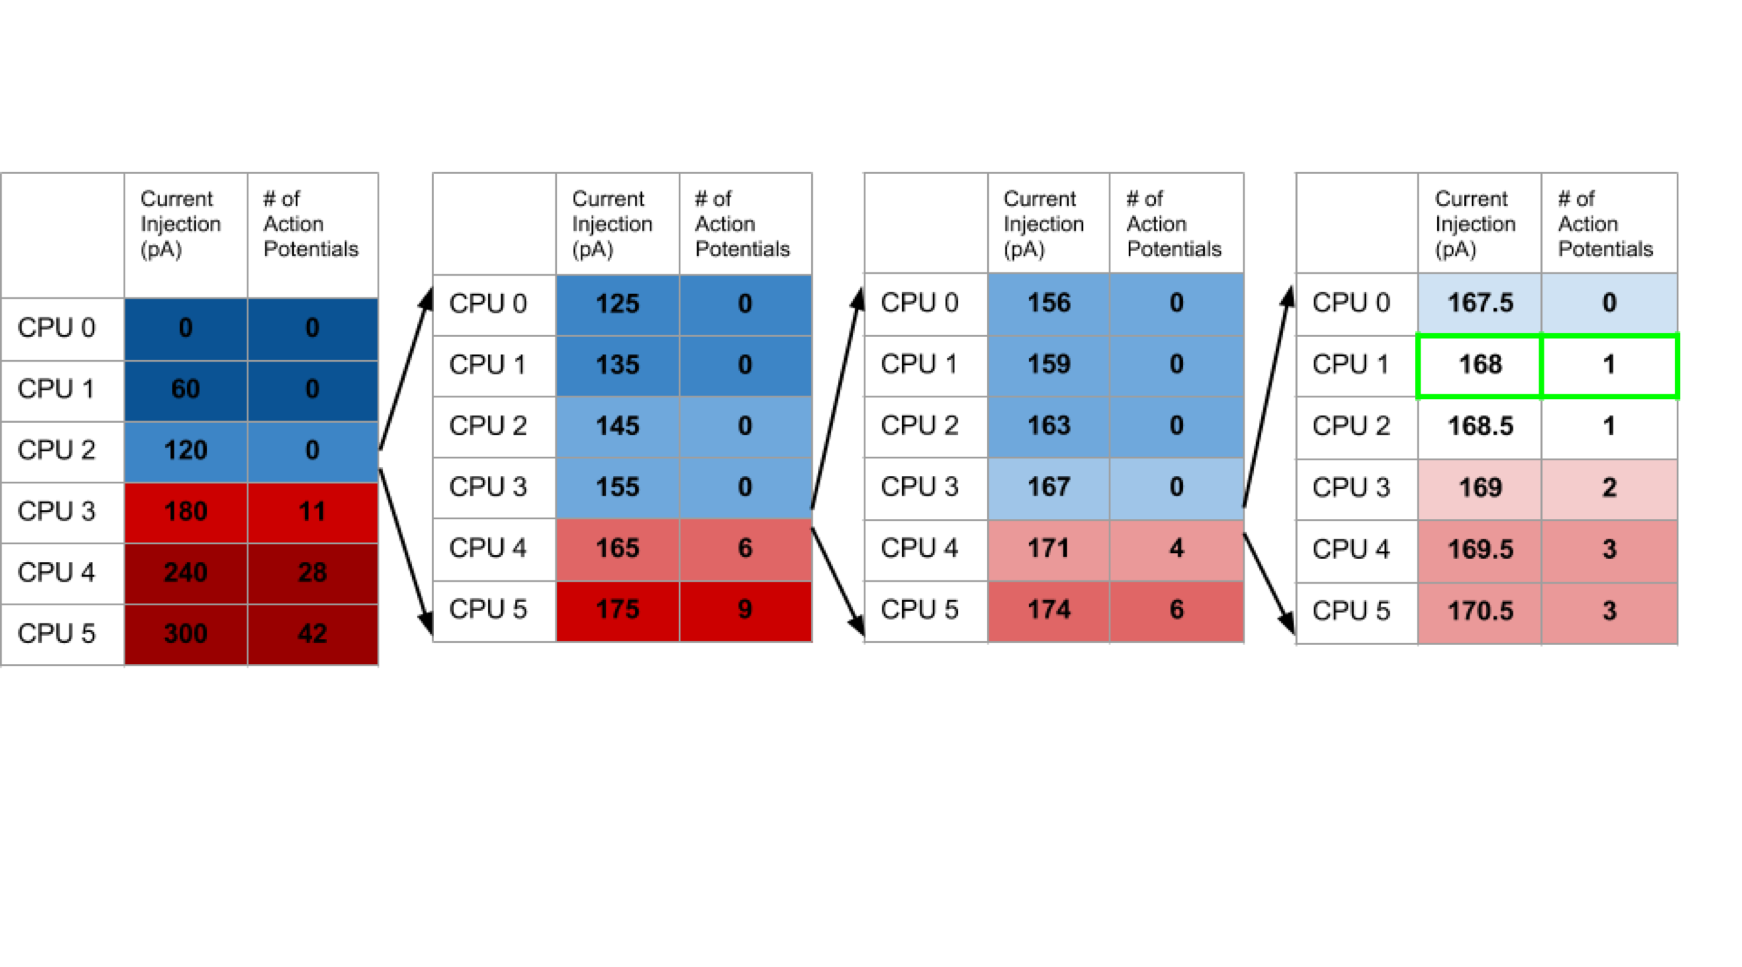
\includegraphics[width=0.7\linewidth]{{figures/rheobase_algorithm.png}}
    \caption{We developed a generic algorithm which took models, and found the minimal current injection value that would cause only one spike. The normal structure of this algorithm is a binary search, however we modified the algorithm so it would map onto multiple processors at once. This lead to significant speed ups for multicompartment NEURON models}
    \label{fig:rheobase}
  \end{center}
\end{figure} 
    
\subsection{Practical application}
I benchmarked this approach using simulations of multi-compartment neuron models.
The parallel rheobase determination algorithm resulted in a significant speed up relative to the serial algorithm.
To amplify the effect, I also considered a scenario where one wants to learn the value of the rheobase with much more precision (down to small fractions of a pA), for example in studies of dynamics in the neighborhood of a bifurcation where all other state variables can be considered nearly unchanged in the sub- and suprathreshold scenarios.
To achieve such precision, i.e. for such a small value of $i$ $0.0001*pq.fA$, the number of simulations $log_2(I/i)$ may be ~20.
Since additional model features may require only a few additional simulations to extract, it is clear that in this scenario the rheobase completely dominates the bulk of the total simulation budget.

In this scenario, using only 16 threads (with a theoretical speedup of $log_2(16+1) ~ 4.09$), I achieved the following results:
\begin{verbatim}
NEURON simulation of multicompartmental model
Serial Rheobase determination: 18.7 s
Parallel Rheobase determination: 4.8 s
Speed up = 3.9x

Brian2 simulation of AdEx model
Serial Rheobase determination: 0.791 s
Parallel Rheobase determination: 0.259 s
Speed up = 3.0x
\end{verbatim}

The total speedup approached but fell a bit short of the theoretical speedup due to overhead in the parallel search algorithm itself.
As the complexity of each simulation increases, and as the number of CPU cores brought to bear increases, this overhead should become a vanishingly small fraction of the total rheobase determination time.

\subsection{Generalization to target spike counts}
This approach determining rheobase was also generalized into a more fundamental algorithm for determining the amplitude of current required to generate a target number of action potentials.
In other words, it can be used to invert points along a models "F-I" function.
\url{https://github.com/russelljjarvis/neuronunit/blob/master/neuronunit/tests/target_spike_current.py}.

\section{Electrophysiological Measurement Distributions From the Experimental Literature}
\label{sec:data-sources}
Organized, publicly available electrophysiological measurements from single, biological neurons can form an optimization target.
Together, they can be used to parameterize a suite of tests against which a model is optimized.
Optimization aims to find model parameters so that electrophysiological measurements based on model simulations are as similar as possible to those observed in neurons.

\subsection{NeuroElectro}
\label{sec:neuroelectro}
One general source of such experimental measurements is The NeuroElectro Project \citep{tripathy2014neuroelectro}, which contains experimental values for 47 distinct electrophysiological measurements across 235 different neuron types.
As with most of the data discussed here, most (but not all) of these measurements were obtained from slice physiology experiments in rodents.
These measurements were programatically extracted from peer-reviewed journal articles over a $\sim20$ year period from $\sim1990-2012$,
and are made easy to access by an application programming interface (API) that NeuronUnit provides bindings to.
Importantly, the measured values--even for a single neuron type--reflect experiments done in many labs using (in some cases) variable methods.
Therefore, the mean of these values (e.g. the mean input resistance across reported Purkinje cells) averages over heterogeneity across cells within a slice, slices within an animal, animals within a lab, and labs within the field.
The sample size for one measure (e.g. input resistance) may be larger than for another (e.g. resting potential) meaning that these measures may reflect different subsets of experiments.
With those caveats in mind, NeuroElectro remains the most direct way to get a large number of optimization-constraining data values for most neuron types.

In order to verify that the data from NeuroElectro was plausible and was being captured correctly for the purposes of the work in this thesis, I used the API along with a batch visualization pipeline to visualize the distributions of electrophysiological measurements and inspect them for a) quality control and b) evidence of multimodality.
Multimodality, meaning multiple peaks in the histogram of a single measurement type for a single cell, could be evidence of a physiological heterogeneity not easily explained by random measurement error.
Two peaks in the histogram, for example, could result from two distinct subclasses of a single nominal neuron type, each with its own (narrower) distribution of the same measurement.
In some instances, the mean and standard deviation alone described the measurement distributions well, as would be expected for random, normally-distributed measurements of a single cell type under reasonably consistent conditions.
These values were then ``approved" for use in model-fitting.
In other cases, these conditions were not met, as exemplified in the figures below.

%\begin{comment}
%\begin{figure}
%\centering
%   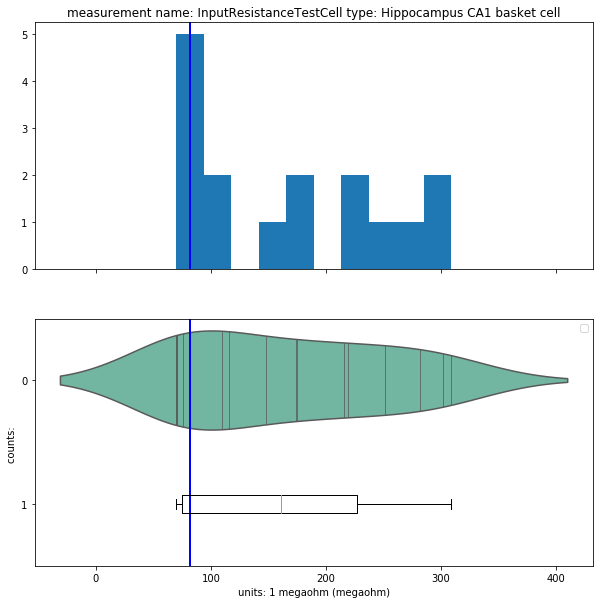
\includegraphics[scale=0.8]{notebooks_converted/needata_thesis_files/needata_thesis_5_5}
%\end{figure}

%\caption{Model parameterization of the brian2 simulator with the customization: interpolated spike height, forced to be above $0mV$}
%
%  \label{fig:sub1}
%\end{subfigure}%
%\begin{figure}
%\centering
%  \includegraphics[scale=0.8]{notebooks_converted/needata_thesis_files/needata_thesis_5_6}
%\end{figure}

%    
%    %\caption{Default model parameterization of the custom written integrator}
%  \label{fig:sub2}
%
%\begin{subfigure}
%  \centering
%      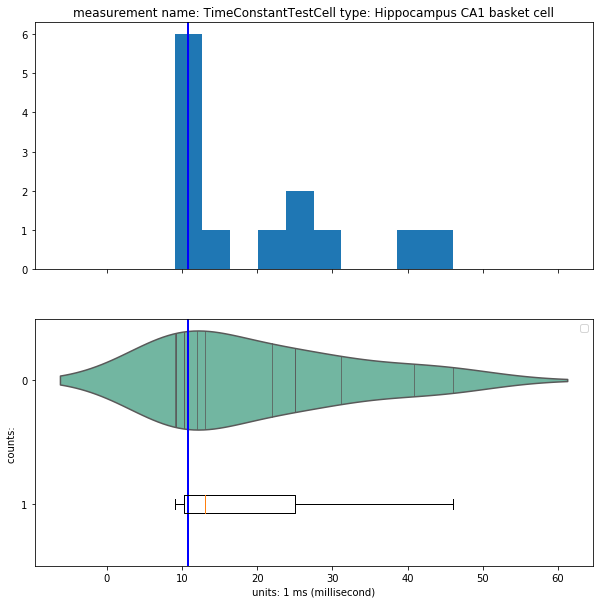
\includegraphics[scale=0.8]{notebooks_converted/needata_thesis_files/needata_thesis_5_7}
%      %\caption{Default model parameterization of the custom written integrator}
%  \label{fig:sub2}
%\end{subfigure}
%
%\caption{Comparison between two Adxaptive Exponential Implementations}
%\label{fig:test}
%\end{center}
%\end{figure}
%
%\end{comment}

%\begin{center}
%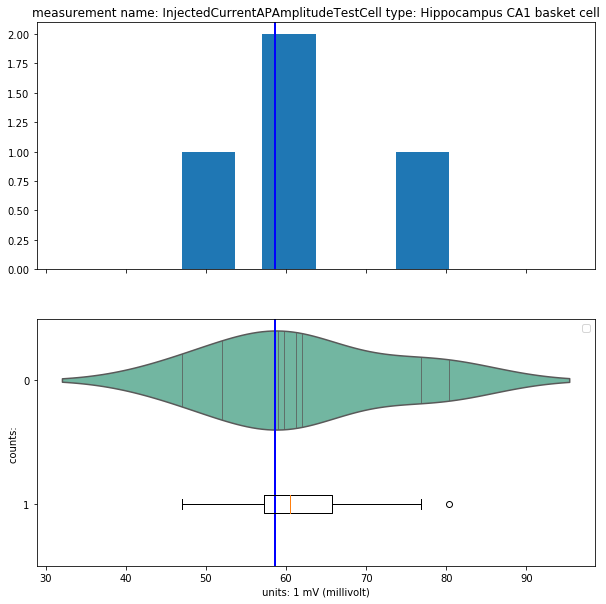
\includegraphics[width=0.7\linewidth]{notebooks_converted/needata_thesis_files/needata_thesis_5_8}
%\end{center}
%
For the majority of cell types and electrophysiological features, the distributions obtained from NeuroElectro were well-described by a normal (or log-normal) distribution.
However, I manually identified and labeled those cases where the data were not well-behaved, as these cases are likely to produce optimized models that do not reflect anything of biological relevance.

Methods for verifying that a distribution is unimodal exist \citep{maechler2013package}; however, rather than entrust this job to top-down automation, I decided to apply my own human knowledge of statistics in order to assess each distribution individually. %, because there seemed to be less opportunity to suffer from some kind of machine introduced violation of intuition. % too each  

%I achieved greater quality control through visual inspection of each case in a piece-meal manner. % manually means to do something by hand. 
I estimated that across all NeuroElectro data sampled here, about $2/3$ of distributions are well represented by a unimodal and normal distributions (e.g. Figure \ref{fig:normal-feature}).
In the remaining $1/3$, where this did not hold, I observed a small but still significant number of odd cases: highly skewed distributions (Figure \ref{fig:skewed-feature}), bimodal distributions (Figure \ref{fig:bimodal-feature}), uniform-like distributions, and distributions with insufficient samples to make any judgement.

\begin{figure} 
    \begin{center}
   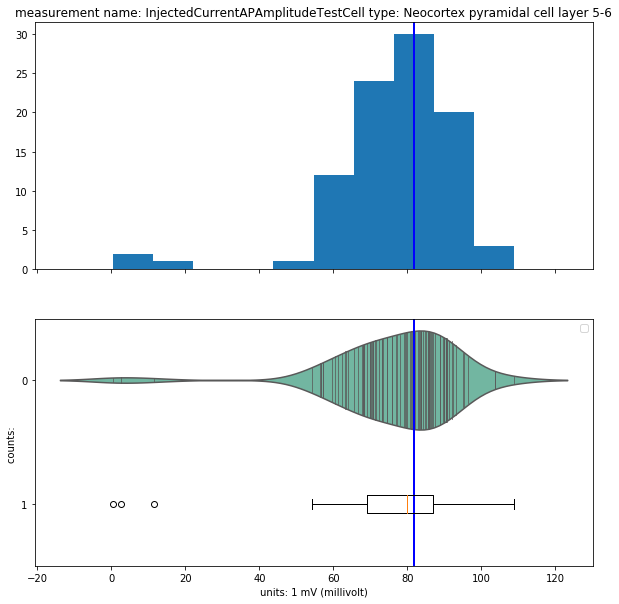
\includegraphics[scale=0.8]{figures/mean_well_served.png}
   \caption[AP Threshold Data Distribution for Layer 5 Pyramidal Cell]{\textbf{AP Threshold Data Distribution for Layer 5 Pyramidal Cell.} The majority of NeuroElectro data sets followed a normal distribution, where the mean is surrounded by a very high density of samples, which slowly thin out with increasing distance from the mean. The distribution is approximately symmetrical. Top Panel: A histogram of AP Threshold measurements from Layer 5 Pyramidal Cells; Bottom Panel: A violin plot and a box plot summarizing the same distribution. In this plot, the mean and mode are close together (a necessary condition for near-normality).
   Analagous plots were generated and inspected for all electrophysiological features computed here.}
   \label{fig:normal-feature}
    \end{center}
\end{figure}   

%\begin{figure} 
%    \begin{center}
%    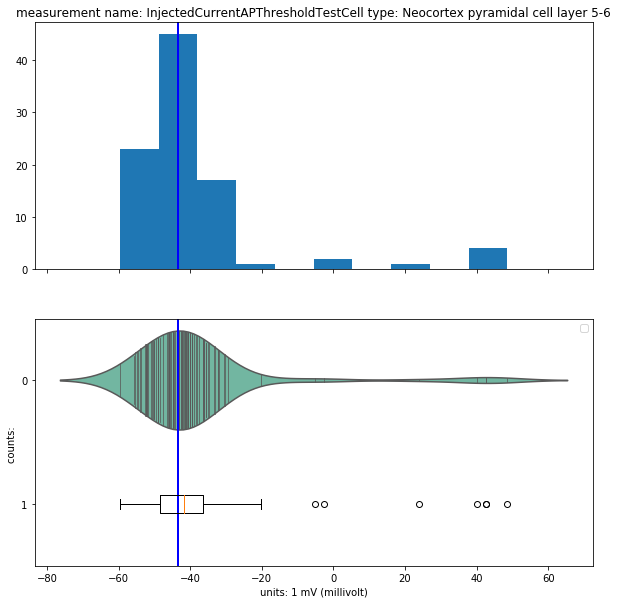
\includegraphics[scale=0.8]{figures/mean_well_served2.png}
%    \end{center}
%    \caption[AP Amplitude Data Distribution for Layer 5 Pyramidal Cell]{\textbf{AP Amplitude Data Distribution for Layer 5 Pyramidal Cell.} Same as the figure above, but for the AP Amplitude.}
%    \label{fig:normal-feature2}
%\end{figure}   
 
\begin{figure} 
    \begin{center} 
    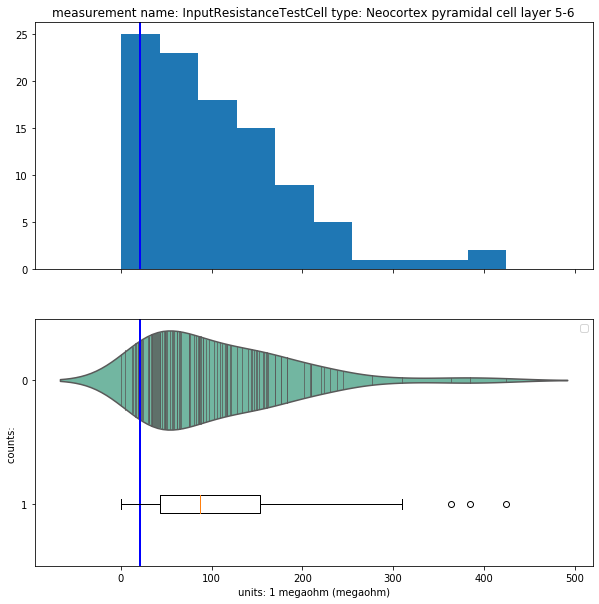
\includegraphics[scale=0.8]{figures/skewed_distribution.png}
    \end{center}
    \caption[Example of Skewed Distribution]{\textbf{Input Resistance Data Distribution for Layer 5 Pyramidal Cell.} Similar to Figure \ref{fig:normal-feature}, except for Input Resistance.
    Unlike in that figure, the distribution shows a strong skew towards higher values.
    The mean and the mode are no longer well-aligned, and therefore the mean is no longer representative of the most typical value of this feature for this neuron type.}
    \label{fig:skewed-feature}
\end{figure}   

%\begin{figure} 
%\caption[NeuroElectro data - uniform distribution]{}
%    \begin{center}
%    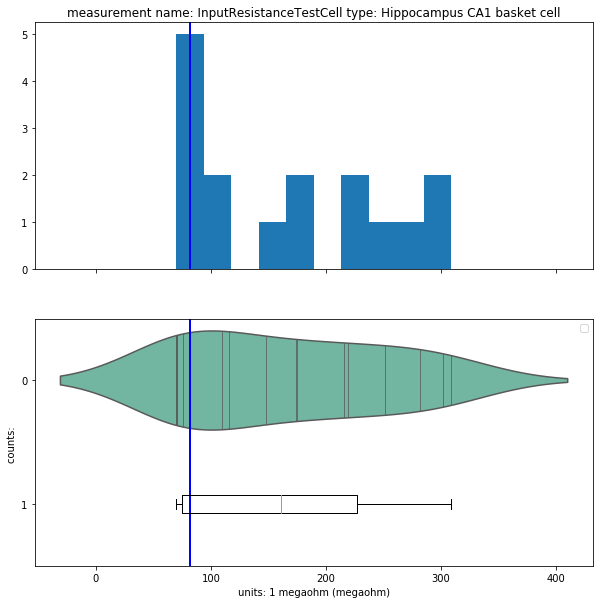
\includegraphics[scale=0.8]{figures/uniform_distribution.png}
%    \end{center}
%\end{figure}       
%%
% Neuronunit code handles under sampled neuroelectro code.
%\begin{figure} 
%\caption[NeuroElectro data - undersampled distribution]{}
%    \begin{center}
%    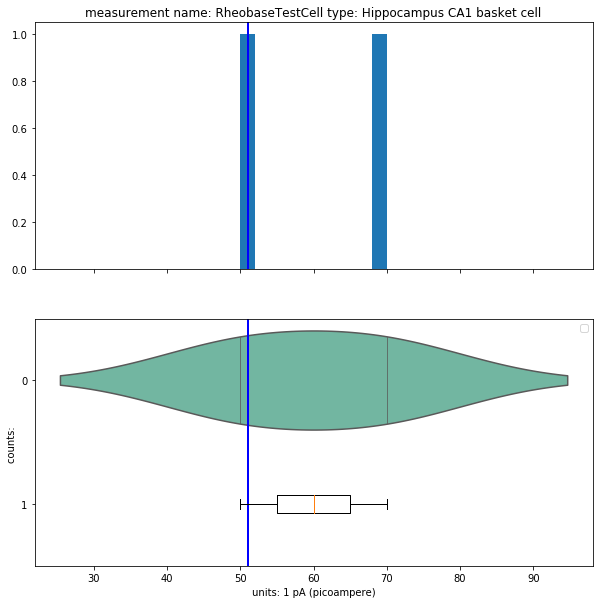
\includegraphics[scale=0.8]{figures/undersampled_distribution.png}
%    \end{center}
%\end{figure}   
%%
    
%\begin{figure} 
%    \begin{center}
%   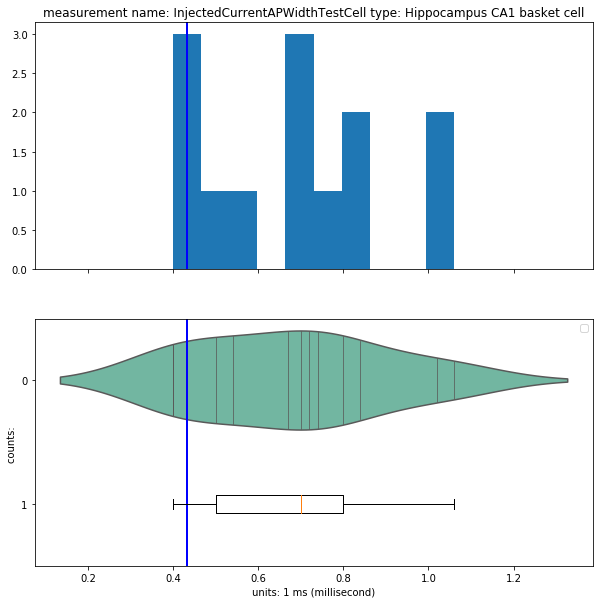
\includegraphics[scale=0.8]{chapters/notebooks_converted/needata_thesis_files/needata_thesis_5_9}
%   \caption{The Action Potential Width of the Hippocampus CA1 basket cell possibly has either an underlying uniform distribution or a multimodal distribution. Since the samples are few, the true distribution is unknown. If the distribution is uniform the gaps in the distribution, that give the histogram a multimodal appearance, as the sample size is lower enough that such gaps may only represent missing samples.}
%    \end{center}
%\end{figure}


%\begin{figure}   
%\begin{center}
%   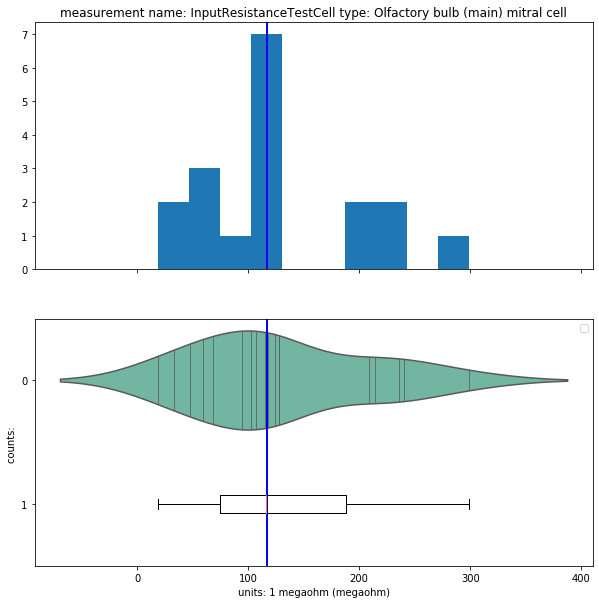
\includegraphics[scale=0.8]{chapters/notebooks_converted/needata_thesis_files/needata_thesis_5_21}
%         \caption[Input Resistance Olfactory Neuron, Perhaps Bimodal]{Input resistance of the Olfactory Mitral cell showed some tendency towards underlying bi-modal distribution, however in the second block of histogram bins, centered around $200-300pA$ only contains approximately $5$ samples. Due to a lack of samples it is also possible to conclude that the data belong to an under sampeled uniform distribution. This data set was important, as one Olfactory neuron test was constructed from this data.}
%\end{center}
%\end{figure}
   
\begin{figure}  
\begin{center}     
  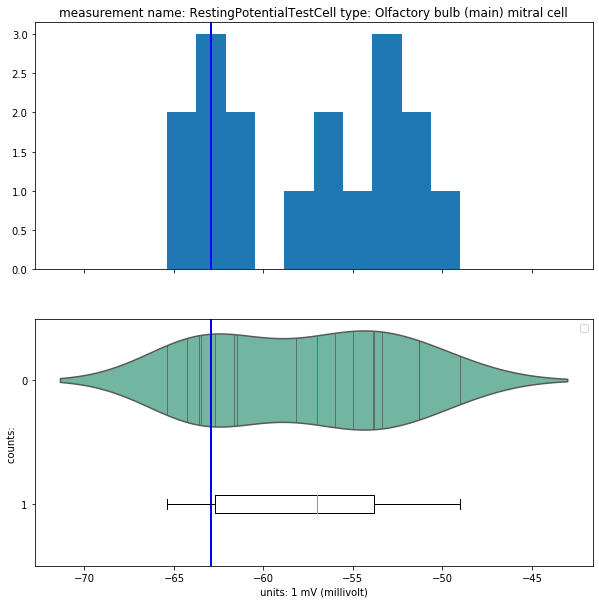
\includegraphics[scale=0.8]{chapters/notebooks_converted/needata_thesis_files/needata_thesis_5_22}
      \caption[Bi-modal Distribution for Resting Membrane Potential from Mitral Cells]{\textbf{Resting Potential Data Distribution for the Olfactory Bulb Mitral Cell.} Similar to the previous figures, but for a different cell type and electrophysiological feature.
      In this case, the distribution is clearly bimodal, with each mode containing a similar density of the data.
      Now both the mean and the median (small red line in box plot) are especially unrepresentative, lying in a region of low probabilty density.
      }
      \label{fig:bimodal-feature}
\end{center}     
\end{figure}
%%
% There are plenty of examples of bi-modal distributions in measurements from cells which are not relevant to this work.
%
%\begin{figure}
%  \centering
%  \includegraphics[scale=0.8]{chapters/notebooks_conv%erted/needata_thesis_files/needata_thesis_5_6}
%   \caption{Default model parameterization of the custom written integrator}
%  \label{fig:sub2}
%\end{figure}
%\begin{figure}
%\begin{center}
%includegraphics{chapters/notebooks_converted/needata_thesis_files/needata_thesis_5_13}
%\end{center}
%\end{figure}
    
%\begin{figure}
%\begin{center}
%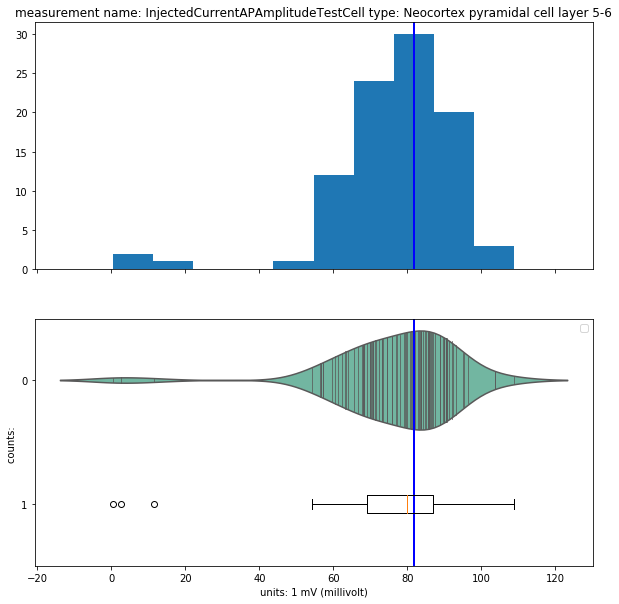
\includegraphics[width=0.7\linewidth]{chapters/notebooks_converted/needata_thesis_files/needata_thesis_5_16}
%\caption[Spike Width Measurements from Neocortical Pyramidal Neurons]{\textbf{Spike Width Measurements from Neocortical Pyramidal Neurons.} (Top Panel) Binned histogram of NeuroElectro spike width measurements from neocortical pyramidal neurons.
%The mode is denoted by the blue vertical line. The mode can be compared to the mean shown in the box plot. Often modes and means of measurements disagree.  NeuroElectro shows that a very common distribution shape is one which is possibly uniform or multi-modal. It is worth noting that a uniform distribution is not well-described by a normal distribution.}
%\label{fig:uniform-feature}
%\end{center}
%\end{figure}

%\begin{figure}
%\begin{center}
%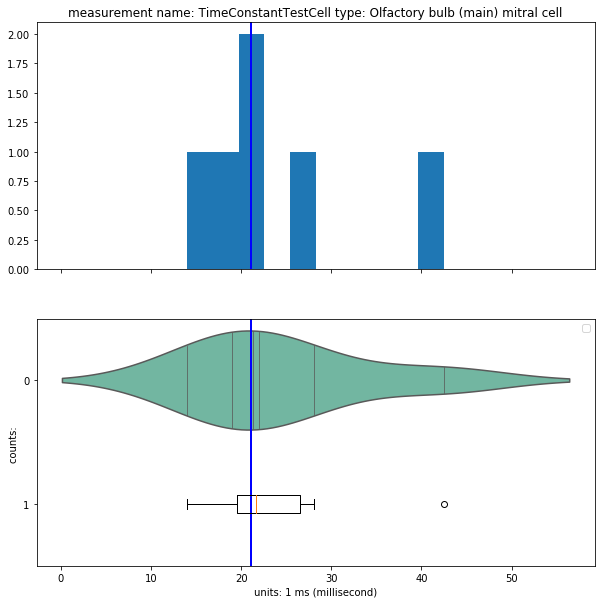
\includegraphics[scale=0.8]{chapters/notebooks_converted/needata_thesis_files/needata_thesis_5_23}
%\caption{Similar to the figure above, but for a different neuron type.}
%\label{fig:uniform-feature2}
%\end{center}
%\end{figure}

\subsection{EFEL and The Allen Institute Cell Types Database}
The Electrophysiology Feature Extraction Library (EFEL) \citep{EFEL} was developed as part of the Blue Brain Project. Although EFEL computes common spike train statistics related to spike timing, approximately 2/3rds of features extracted by EFEL pertain to spike shape, where some of these features are shown below. 
The Allen SDK comes with a very comprehensive Python-based feature extraction suite. Like EFEL, the Allen suite well-represents a large number of spike shape measurements as well as spike train statistics. 
Unfortunately, the Allen SDK feature extractor is significantly slower than EFEL, as EFEL was implemented using the very fast language $C++$. The performance cost may not be felt when dispatching single runs, but slow performance is a significant impediment to optimization. 
In optimisation, feature extraction is directly coupled to chromosome fitness calculations, and it is executed very often across the evolution of the genetic algorithm. Additionally by default, the Allen SDK feature extractor assumes that the user will apply very high sample frequency and noisy traces encoded in the NeuronData Without Borders \citep{teeters2015neurodata} standardized format. 
These traces require filtering before computing the Allen features, where significant intervention is required to turn off filtering. 
Inappropriately applying filtering to model traces causes problems, because the the lower sampling frequency intrinsic to simulated model traces is not predicted by the digital filter. Overall, the EFEL was fast enough to be useful, and its default settings were appropriate to my use case \citep{garcia2014neo}.

Data available through NeuroElectro cover a large number of cell types; however, recording conditions and measurement algorithms are heterogeneous.
It is unclear whether the distribution of measurements across such an ensemble is actually a good summary of any one individual neuron.
In order to ensure that reduced models could be optimized against data recorded exclusively from single neurons, I also used data from the Allen Institute Cell Types Database \citep{celltypes}, a project of the Allen Institute for Brain Science.
This Cell Types database consists of summary physiological, morphological, and histological data for thousands of individual neurons (across a few dozen subtypes) from mouse visual cortex, obtained using patch clamp recordings in slices.
Each experiment is done using exactly the same methods and with the same sequence of stimuli \citep{celltypes}, ensuring not only that models generated using this data are directly comparable, but that each such model is reflective of an individual neuron.

The Cell Types Database provides some limited pre-computed measures of action potential waveform characteristics. 
However, the data are not organized in a way that makes it is useful for the types of optimization and data analysis performed here.
Specifically, I require features that are computed on cell responses to current injection values that are fixed multiples of rheobase.
Additionally, the pre-computed features are thin relative to those that used for the optimizations described in the Results section.
Because raw data are available through the Cell Types API, I re-computed all necessary features from this raw data, according to the consistent standards reflected in the NeuronUnit code.

In contrast to NeuroElectro, the Cell Types database also has a great deal more information relevant to the above threshold dynamics of neurons, such as the number and pattern of action potentials they discharge in response to somatically-injected currents much larger than rheobase, or in response to non-square injected currents.
In order to exploit these, I developed several additional NeuronUnit tests using EFEL (describe later in sections \ref{sec:efel}), such as: ``time to first spike test", ``mean AP amplitude test", ``time to last spike test" and ``adaption index". In principal any feature measured in the Cell Types Data could be upgraded to a NeuronUnit test, and I created a code-generation template to accelerate this task. Effectively, code generation meant, that any EFEL feature, could be turned into a NeuronUnit test. In principle Allen tests can be generated from templates in much the same way. The final set of operational tests
were EFEL \cite{EFEL} tests that were adapted from descriptions of feature extraction in the literature and shown in Table \ref{tab:features}. 
Features are shown in Figures \ref{fig:voltage_figures} and \ref{fig:features_example}.
I also crafted additional NeuronUnit tests to supplement these including one that measures the slope of the FI curve ($FISlopeTest$) and one that measures the coefficient of variation of the ISI distribution for suprathresholds stimuli ($ISICVTest$), a measure of burstiness. 
%%
% \ref{sec:allensdk},
% Allen are features, not tests (no judge methods).
% currently, its very transient.
% Allen used to be tests, it was hard to % maintain code. 

%%%
% Tests I rewrote from scratch 
% not EFEL, was FITest, CVTest, ISITest
%%%


%\begin{figure}
%\centering
%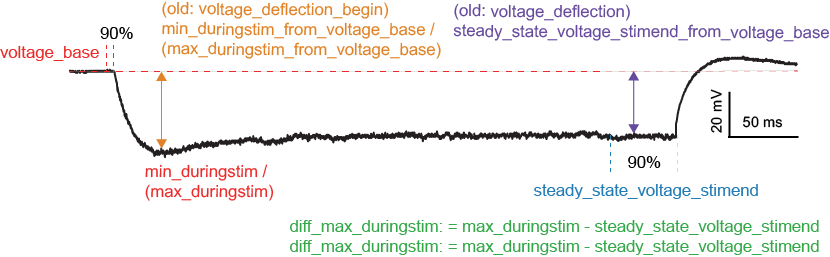
\includegraphics{figures/voltage_features.png}
%\caption[Passive Membrane Properties Measured from a Hyperpolarizing Current Stimulus]{\textbf{Passive Membrane Properties from a Hyperpolarizing Stimulus.} Applying a negative (outward, hyperpolarizing) current stimulus minimially activates voltage-dependent ion channels, making it a good method for measuring ``passive" membrane properties such as the input resistance (measured as the difference between the resting potential (red) and steady-state hyperolarization (blue).
%Nonetheless, some intrinsic conductances are activated, allowing for measurment of additional features such as the sag ratio (red trough vs blue steady state). Figure from EFEL documentation \url{https://efel.readthedocs.io/en/latest/eFeatures.html}.}
%\label{fig:voltage_figures}
%\end{figure}

\begin{figure}
\begin{center}
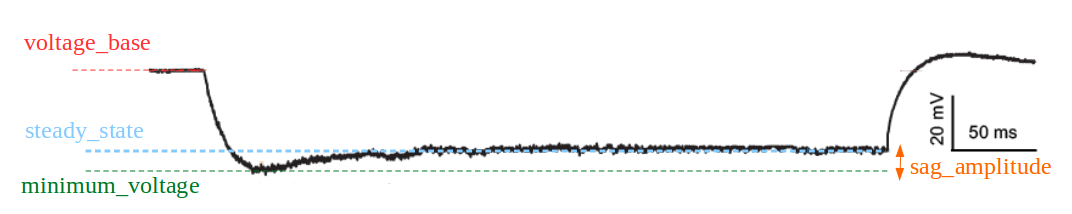
\includegraphics{figures/sag_amplitude}
\end{center}
\caption[Passive Membrane Properties Measured from a Hyperpolarizing Current Stimulus]{\textbf{Passive Membrane Properties from a Hyperpolarizing Stimulus.} Applying a negative (outward, hyperpolarizing) current stimulus minimially activates voltage-dependent ion channels, making it a good method for measuring ``passive" membrane properties such as the input resistance (measured as the difference between the resting potential (red) and steady-state hyperpolarization (green).
Nonetheless, some intrinsic conductances are activated, allowing for measurment of additional features such as the sag amplitude or ratio (green trough vs blue steady state). Figure from EFEL documentation \citep{efel-docs}.}
\label{fig:voltage_figures}
\end{figure}

\begin{figure}
\centering
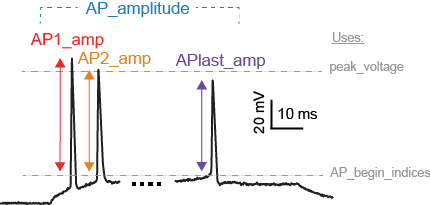
\includegraphics{figures/AP_Amplitude.png}
\caption[Action Potential Features Measured from a Depolarizing Current Stimulus]{\textbf{Action Potential Features Measured from a Depolarizing Current Stimulus.} A positive (depolarizing, inward) current of sufficiently amplitude produces one or more action poentials.
Many features can be computed from these, including their absolute amplitudes (in color), relative amplitudes, widths, thresholds, and afterhyperpolarizations (AHPs).
Additional features about their number and relative timing can also be computed (not shown).
Figure from EFEL documentation \citep{efel_documentation}.}
\label{fig:features_example}
\end{figure}



%XXXX Russell, can you list the new tests above.

These tests can be used to assess the agreement between neuron models and biological neurons on supra-threshold dynamics, largely reflected in patterns of spiking such as bursting and adaptation, but also mean spike height and mean spike width, resting membrane potential, mean trough depth, and upstroke times.

\subsection{The Blue Brain Project Neocortical Microcircuit Portal}
\label{sec:bluebrain-data}
I also made use of an additional data source, the The Blue Brain Project Neocortical Microcircuit Portal, similar in some ways to the Allen Institute Cell Types Database but reflecting measurements taken from mouse somatosensory cortex (again in patch-clamp recordings from slices).
From this dataset I exclusively used a collection of experiments from animal $B95$, which for reasons unknown yielded a tremendous amount of data \citep{ramaswamy2015neocortical}.
Conceptually, this dataset did not add anything new, but it did allow for high-quality optimized models to be produced from another brain region (somatosensory, rather than visual cortex).
These data are also linked to--and constrain--the on-going Human Brain Project effort to simulate biophysically-detailed multi-compartmental models of the same neurons (and whole neural circuits).
This means that the reduced models produced here can be compared directly to those more detailed models, or that the general NeuronUnit-driven genetic optimization framework developed here could be used to optimize detailed models which should, in principle, be similar to those produced through the larger Human Brain Project effort.
Indeed, the Human Brain Project is already a user of the SciUnit framework developed in my lab, on which NeuronUnit is based.

\begin{table}
\centering

\resizebox{\textwidth}{!}{
\begin{tabular}{|l|l|}
            \toprule
            \textbf{Test Name} & \textbf{Test Description}\\
\midrule
adaptation-index & Measures spiking fatigue in response to constant current\\
 adaptation-index2 & The same as Adaption index1, except it is used as an alternative when spikes below $0mV$ occur.   \\
time-to-first-spike & amount of time elapsed until first spike \\ mean-AP-amplitude & The average spike height in a spike train \\
spike-half-width & The width of a spike is obtained at point when spike height is half its total amplitude\\    
AHP-depth & The after hyperpolarisation depth\\
minimum-voltage & The minimum voltage\\
peak-voltage & the maximum voltage, usually a spike peak. \\
time-to-last-spike & The time of last spike onset \\
AHP-depth-abs & After Hyperpolarisation depth (absolute value).\\
all-ISI-values & All interspike interval times\\
voltage-base & minimum voltage while undergoing stimulus, often below the threshold of APs. \\
min-voltage-between-spikes & Needed because during  high frequency firing AHPs may be skipped.\\
Spikecount & Just the number of spikes that occured in the provided stimulus window\\
\bottomrule
\end{tabular}}
\caption[List of EFEL Features]{14 key features identified in the EFEL \citep{EFEL} library that I impemented and encoded into NeuronUnit tests for optimization.}
\label{tab:features}
\end{table}

% There is no "NeuronUnit" data. What does this mean?
The tests which lead to the best fits in the above threshold experiments were the tests made from application of EFEL features to Allen data sources (Figure \ref{fig:voltage_figures}). The measurement type and the test type did not change between Allen Cell Types and Blue Brain Data. Only the reference data which informed comparison measurements changed. % \ref{fig:supra-threshold-tests})

Table \ref{tab:features} constitutes a summary of both NeuroElectro and Allen experimental data reports. %This data can naturally be reported in tabular form. 

%\subsection{Experimental Measurements}

\begin{table}[ht]
\centering
\resizebox{\textwidth}{!}{
\begin{tabular}{|l|l|l|l|l|l|l|l|l|}
\toprule
Test Name / Cell Type & CA1 Pyramidal & Purkinje & NCP Layer 5-6 &      Mitral Cell & 623960880 & 623893177 & 471819401 & 482493761 \\
\midrule
RheobaseTest                   &                      189.24 pA &                680.79 pA &                          213.85 pA &          NaN &        70.0 pA &       190.0 pA &       190.0 pA &        70.0 pA \\
InputResistanceTest            &                    107.08 $M\Omega$ &              142.06 $M\Omega$ &                        120.67 $M\Omega$ &  130.08 $M\Omega$ &  241.0 $M\Omega$ &  136.0 $M\Omega$ &  132.0 $M\Omega$ &  132.0 $M\Omega$ \\
TimeConstantTest               &                        24.5 ms &                      NaN &                           15.73 ms &     24.48 ms &        23.8 ms &        27.8 ms &        13.8 ms &        24.4 ms \\
CapacitanceTest                &                        89.8 pF &                620.27 pF &                          150.58 pF &    235.75 pF &            NaN &            NaN &            NaN &            NaN \\
RestingPotentialTest           &                      -65.23 mV &                -61.59 mV &                          -68.25 mV &    -58.14 mV &       -65.1 mV &       -77.0 mV &       -77.5 mV &       -71.6 mV \\
InjectedCurrentAPWidthTest     &                        1.32 ms &                  0.41 ms &                            1.21 ms &      1.61 ms &            NaN &            NaN &            NaN &            NaN \\
InjectedCurrentAPAmplitudeTest &                       86.36 mV &                 71.23 mV &                           80.44 mV &      68.4 mV &            NaN &            NaN &            NaN &            NaN \\
InjectedCurrentAPThresholdTest &                       -47.6 mV &                -46.89 mV &                          -42.74 mV &     -38.9 mV &            NaN &            NaN &            NaN &            NaN \\
FISlopeTest                         &                            NaN &                      NaN &                         0.05 Hz/pA &          NaN &     0.18 Hz/pA &     0.12 Hz/pA &     0.18 Hz/pA &     0.09 Hz/pA \\
\bottomrule
\end{tabular}}
\caption[Neuroelectro Data]{Data for 9 tests (features) across 8 cells.
The first 4 cells are specific cell types spanning several brain regions, and the corresponding data comes from neuroelectro.org.
The remaining 4 are single (cortical) cells comes from the Allen Cell Types database, and the features were directly computed using NeuronUnit tests.
``NCP" indicates neocortical pyramidal.}
\label{tab:neuroelectro-data}
\end{table}


\section{Technical Details of the Optimizer}
\label{sec:tech-details}
The sections above describe my innovations in model construction and simulation, as well as the experimental data brought to bear on optimization. These data are used to parameterize NeuronUnit tests, one per measurement type.
For example, input resistance data for one neuron type in NeuroElectro, or one specific neuron in the Cell Types database, is passed to an \textit{InputResistanceTest} defined in NeuronUnit.
This test ``asks" the model to generate a corresponding simulation, measures the input resistance in this simulation output, and then assesses model/data agreement, resulting in a score.
These mechanics have been described at length previously in \cite{omar2014collaborative}, \cite{gerkin_neuronunit}, and \cite{birgiolas2019towards}.

\subsection{Generating and Using Scores}
\begin{figure}
\begin{center}
    \includegraphics{figures/normal_distribution}
    \caption[Z-scores for NeuronUnit Tests]{\textbf{Z-scores for NeuronUnit Tests}. As discussed in the section \ref{sec:neuronunit}, error functions were evaluated with the assistance of the \emph{NeuronUnit} library.
    This involves obtaining an experimental distribution over electrophysiology feature measurements for a cell type, measuring corresponding model output features, and then locating those features in that experimental distribution. 
    Scores that are closer to the experimental mean are identified as low error.
	The Z-score encodes this information; a Z-score of 0 is the lowest possible error.}
	\label{fig:normal-dist}
\end{center}
\end{figure}
%XXXX Something about Z-score vs RatioScore.

One way to ask whether the simulated feature is a good match to the biological data distribution is to use a Z-score.
The Z-score is defined as:
\begin{equation}
Z-Score = \frac{s - b_{\mu}}{b_{\sigma}}
\end{equation}
where $s$ is the value of the feature in the model simulation, and $b_{\mu}$ and $b_{\sigma}$ are the mean and standard deviation of that feature in the biological data distribution.
The Z-score does not specifically assume that the biological data are normally distributed, although this generates the most natural interpretations.
%(Figure \ref{fig:normal-dist}).
In cases when the biological data from one neuron type comes from a single experiment on a single neuron (as with some data from the Allen Cell Types database or the Blue Brain Project), there is no mean or standard deviation, so I compute a \emph{RatioScore}:
\begin{equation}
Ratio-Score = \frac{s}{b}
\end{equation}%%%Fixed error
where $b$ is the observed biological feature value.
Both types of scores were then normalized to produce an error signal in the range $(0, \inf)$ for use by the optimizer.
For example, suppose a feature(e.g. the rheobase current) had value $\mu \pm \sigma = (100pA \pm 40pA)$ in the biological data, and $110 pA$ in the simulated model output.
Then the following steps were taken to transform it into an error signal:
\begin{enumerate}
 \item A Z-score is computed: $\frac{110 pA - 100 pA}{40 pA} = 0.25$
 \item This is converted to the range (0, 1) using the error function: $abs(erf(Z)) = 0.27$ 
 \item The logarithm is computed: $\log_{10}(0.27) = 0.56$ 
\end{enumerate}
The value 0.56 above represents a larger model/data disagreement than the ``best" possible value of 0 (corresponding to a Z-score of 0), but less disagreement then the ``worst" possible value of $\inf$ (truncated in practice at 100) representing a Z-score of $+\infty$ or $-\infty$. The summed error signal over all $n$ NeuronUnit tests (e.g. rheobase, input resistance, spike rate adaptation, etc.) is:
\begin{equation}
Total  Error = \sum_i^n error_i
\end{equation}
i.e. the sum of all of the errors.  Again, 0 would represent perfect model/data agreement across all tests.

While the optimizer attempts to minimize the total error of the model according to the equation above, evaluation of the quality of the optimized model is evaluated using a hypothesis testing framework.
Specifically, I ask whether there is sufficient evidence that the optimized model is representative of the distribution of feature values observed in the biological data.
The null hypothesis can be states as ``the observed features of the optimized model were drawn from the distribution of features of biological neurons".
In order to generate a test statistic for hypothesis testing, I compute $\chi^{2}$, defined as (in the case of Z-scores):
\begin{equation}
\chi^{2}=\sum\limits_{i=1}^{n}(Z_{i}^{2})
\end{equation}
This equation arises from the fact that a Z-score is simply a standardized normal variable, and a chi-squared distribution with $n$ degrees of freedom is simply the distribution of $n$ independent, squared normal variables.
I compute a p-value by comparing the observed $chi^2$ statistic to the cumulative distribution function of the $chi^2$ distribution with degrees of freedom equal to the number of NeuronUnit tests used (which is equal to the number of Z-scores produced).
If this p-value is small (e.g. $<0.05$), that can serve as evidence to reject the null hypothesis, indicating that the optimized model did not ``fit in" well with the observed biological data.
In contrast, failure to reject the null hypothesis would suggests that the optimized model was somewhat convincing in its mimicry of a biological neuron, for the features in question.

\subsection{Mechanics of Optimization using NeuronUnit}
Here I will describe how I generate these scores concurrently for many parameterizations of the same model and how they guide the optimization path.
I created two different optimization code bases based on the DEAP Python package for genetic optimization \citep{DEAP_JMLR2012}, one that relied on DEAP directly, and one that relied on the BluePyOpt package produced by The Human Brain Project \citep{bluepyopt} (These have since been merged together), in order to achieve optimization using NeuronUnit.
A few key modules are essential to both approaches.
I wrote the file \emph{optimization-management.py} to contain the logic of and methods for managing complex optimization jobs.
It helps the optimizer handle both fixed and varying  model parameters, contains methods for random sampling of model parameter spaces, can plot models output for visualization of this space, and assists in computing the F-I curve.
I also add several methods for inter-converting between representations of the models themselves and the chromosomes that represent only parameter values.

A created a \emph{NUFeature\_standard\_suite} class to convert NeuronUnit features to BluePyOpt objective functions, as outlined in simpler terms in the enumerated list above.
These classes contain a complicated nesting of fault handling statements, as there are many reasons why a candidate model could return unusable simulation output (typically non-biological parameter values), resulting in values like $NaN$ and $\inf$; such values must be recast as poor but finite errors so that the optimizer can see a smooth error surface.
There are two flavors of \emph{NUFeature\_standard\_suite}, one for supra-threshold simulation experiments and another for at threshold or sub-threshold experiments, since each experiment type produces different feature requiring different feature extractors, and producing different sets of edge cases to be handled independently.
For example, there are more ways for a model to fail to elicit multiple action potentials (causing all ISI-based feature extraction functions to return $NaN$ values), than there are to fail to exhibit a hyperpolarizing response to a small outward current injection for the measurement of input resistance.
 
I created a \emph{model-parameters.py} file, a collection of ordered dictionaries, that informed the optimizer which parameters should be modifiable (in the highest-dimensional cases, all of them) and what are reasonable (biologically plausible) search boundaries.
This file also contains example parameter sets representing notable dynamical regimes, such as those shown in \cite{izhikevich2003simple}.
I also made this file and its methods inter-operable with BluePyOpt model parameter management scheme.

\subsubsection{Optimization Parameters}
Optimization requires searching for better and better solution across multiple generations of chromosomes (parameter sets), as noted in section \ref{sec:genetic-algorithms}.
Robust optimization for the models used here required $NGEN\sim150$ generations with a population size (number of parameter sets explored in each generation) of $\mu=35$.
In other words, it took about $150$ generations of mutation, crossover, and selection to achieve convergence, and in each generation about $35$ models had each of their feautures computed and scored.
These parameter values achieved an acceptable balance between exploration of the parameter space and exploitation of favorable regions.
In some cases, values as small as $NGEN=10$ and $\mu=10$ were tolerable, for example when optimizing only low-dimensional cross-sections of parameter space.
In other cases, such as when the number of optimization objectives (i.e. the number of electrophysiological features being tested) was $NOBJ>25$, values as high as $NGEN=300$ and $\mu=100$ were required to obtain adequate results.

\subsubsection{Multiobjective Scoring and Selection}
One potential scientific goal is to maintain a diverse set of solutions (i.e. very different parameter sets that nonetheless each produce simulations that adequately match observed experimental measurements).
The optimization literature has developed many competing approaches for doing this \citep{deb2000fast}, but it usually involves two popular algorithms, named IBEA and NSGA2, which I investigated here.
NSGA2 uses some additional ranking mechanisms, to re-weight the perceived fitness of each chromosome and influence the probability that it survives (or is bred into) the next generation.
For example, it tries to minimize ``crowding distance", penalizing chromosomes that aggregate in clusters, as persistent cluster formation means that the GA becomes preoccupied with more limited regions of the solution space, harming solution diversity.
Another meta-constraint called ``non-dominated sorting" ranks most highly each chromosomes that is not unanimously defeated by any other chromosome on any feature score.
For example, though one parameter set $P$ might produce a model which score poorly on all features except Input Resistance, if no other parameter set has a higher-scoring Input Resistance feature then $P$ is retained. Consistent with personal communication with \cite{van2007neurofitter}, adding in crowding distance and non-dominated sorting typically harms optimizer performance, in the context of neuronal model optimization, though the reason for this is not argued conclusively, I speculate on a likely cause in the discussion of this work.
A simpler ``select best" algorithm (labelled IBEA) dispenses with these tricks, performs no meta-constraint scoring, and simply retains the fittest chromosomes for mutation, crossover, and selection. This simpler selection algorithm was found to work well when optimizing reduced neuronal models.

\subsection{Comparison to Previous Approaches to Optimization}

\subsubsection{Time-dependent Mutation}
Other labs have previously developed schemes to optimize neuron models, e.g. \cite{druckmann2007novel}.
I retained the conceptual insights of these approaches where they were useful for the problems at hand.
For example, I utilized a time-dependent mutation magnitude ($\eta$).
The idea is that big mutations are more helpful in the early stage of optimization, when it is important to explore the vast hyper-volume of parameter sets and get a general picture of the error surface, and that these mutations should be smaller during the later ``refinement" stage of optimization, as the best solutions are approached. Time diminishing $\eta$ did improve genetic algorithm on reduced model optimization problems.

\subsubsection{Variants on Somatic Current Injection}
Nearly all neuron optimization work (including this one) relies on the responses to somatically-injected current as the domain for optimization.
This is largely motivated by the existence of a common and simple experimental analogue using patch clamp (which drives experimental design for both the Allen Cell Types Database and The Blue Brain Project).
But there are three different strategies for choosing the subset of these experiments that are recapitulated in optimization.

% The first strategy was to assume that measurements of an at threshold rheobase spike were sufficient to fit the model to the entire F-I curve, and if all neurons showed an identical regular, non-accommodating spiking pattern, this strategy would might be sufficient to identify a model, with all the right at threshold and above threshold dynamics. To the extent that this assumption is violated, various additional above-threshold current injections will be needed, these are described in strategies two and three. 

% The second strategy involves first identifying the rheobase currents per model and choosing two extra multiples of rheobase current reserved for further model evaluation. This strategy is more direct and slightly more rapid, but it is inefficient in terms of constraining the model, because all of the "action" in the F-I curve occurs above rheobase, but not too far above rheobase (i.e. not at currents that induce depolarization block).

% The third strategy is like the second, but deliberately samples single above threshold locations on the F-I curve (any location that elicits one spike). It is actually the third strategy that was used to produce multi spiking fits, in this work. 

% The fourth strategy involves making an informed guess to make a fixed set of current amplitudes (e.g. ascending 100 pA steps) from the data and probing the model with these, then comparing model and data within this subset. 

%Here I have described four different strategies for constraining models, 
In the optimization framework I tested many different strategies for constraining models with current injections, there were only two important differences between all four strategies: one type of strategy constrains cell behavior at multiple values of current injection, and the other strategy constrains cell behavior at a single current injection value (rheobase or otherwise). Each strategy seeks to resolve a ``bias variance trade-off" differently, and so knowledge of bias variance trade-off is important for understanding the dramatically different quantities of fit found.

When only one current injection value is used seemingly great fits of spike shape, and spike time can be achieved, because the reduced models are more able be over-fitted with respect to a limited range of data. When a model is constrained relative to multiple current injection values, over-fitting of the model is less possible. The optimizer produces a model that is compromised on almost all constraints, with few exceptions. %Because of design choices in multispiking optimization the main constraint that is robust against being compromised is the current versus firing rate relationship. This result is compatible with other findings in the literature probably many optimizer compromises have lead to spike shape being poorly recovered by the optimizer but spike times are perfectly recapitulated \citep{rossant2011fitting}. 

Deliberately over-fitting models was an important optimization strategy in the earlier development of the optimizer, as at the time the highest priority was to verify that the optimizer was functional in a multi-spiking context, however, now with functionality well established producing less good but more generalized fits will become a higher imperative.

% , but the majority of other fitness values will be heavily compromised
%%
% Not inefficient at constraining model, but efficient at 
%%


%This strategy was used not just in optimization, but also in the analysis and re-organization of existing ephys data.
% Action potential waveforms are most regular and consistent in shape when evaluated very near rheobase. Are they? 

%If one follows a multiple current injection optimization strategy, one must also decide how many current amplitudes (above rheobase) must be evaluated in order to adequately constrain model parameters.

% 

%There is an further issue

% the second and third strategy, 

% It attempts to identify the minimum current required to cause some target spike number observed in a dataset. With matching spike counts across simulated and biological data, downstream feature analysis (e.g. spike rate adaptation indices) are likely to be more directly comparable. The consequences of these decisions are explored in the Results section.


%Differences in spike shape and spike timing statistics are thus only modulated by differences in model parameters.

\subsection{Feature Extraction}
Each NeuronUnit test used in the optimizer represents the evaluation of a single feature of simulated output, for example the Input Resistance.
I greatly extended the number of such features/tests covered by NeuronUnit in order to produce a rich, multi-objective optimizer that could capture important spiking dynamics and to obtain insights into what would be the most compact subset for subsequent use in unique identification of models.

\subsubsection{Elephant Features Test Suite}
\label{sec:elephant}
Elephant \citep{elephant18} provides feature extraction capabilities for membrane potential time series expressed using the Neo library in Python \citep{davison_neo}.
Eight NeuronUnit tests (five used here) are derived from Elephant feature extraction, particularly those associated with passive membrane properties assessed with subthreshold stimuli, or action potential waveform properties assessed at rheobase.
Fundamental quantities such as capacitance or input resistance are among these, though they are not ``emergent properties" of the model since they are roughly predictable from the parameters of the model equations.

\subsubsection{Electrophysiology Feature Extraction Library (EFEL)}
\label{sec:efel}
%Most suprathreshold dynamics were summarized by descriptive statistics of patterns of action potentials. For example, the coefficient of variation of the inter-spike intervals in a spike train can serve as a measure of "burstiness". -- No EFEL has many spike shape qualities. as the noted well as spike train statistics. I'd say the ratio of spike train statistics to spike shape measurements is about 1:1.
The Blue Brain Project developed the Electrophysiology Feature Extraction Library (EFEL) to compute many such statistics from spike trains, and I used these to generate tests of suprathreshold dynamics for optimization \citep{EFEL}.

\subsubsection{Allen Institute Software Development Kit (Allen SDK)}
\label{sec:allensdk}
The Allen Institute offers yet another set of tools for feature extraction, applying to both sub- and suprathreshold features of neuron responses to current injection.
The reason to use Allen features in addition to the above is that some of these features are predicated on particular current stimuli (e.g. a stimulus that is exactly 20 pA stronger than the rheobase current).
% I don't think the following is needed, and it may be misconceived.

% Here is why: In the Allen sweep data sets, the current that produced the voltage is known and stored (think of it as a current V_M pair), it is not thrown out. 

% In any case, if you have Allen data and Allen features, or Allen data and EFEL features. Comparing the original voltage trace is still possible, comparing to the original current is still possible. The main thing that _is_ lost is the opportunity to align findings with official Allen features, but that's it.
Such stimuli either were or were not delivered to the various experimentally recorded neurons, and for the purposes of this thesis there is no going back and delivering additional ones.
Consequently, for model testing and optimization it makes sense to use features--and the stimuli that generated them--that can be directly compared to the recorded neurons.
For the biological neurons in the Allen Cell Types database, these features are available in the Allen SDK.

